\documentclass{ieeeaccess}
\usepackage{cite}
\usepackage{url}
\usepackage{xurl}
\usepackage{lipsum}  
\setlength {\marginparwidth }{2cm}

%workaround for clash of todonotes package, see 

\newcommand{\todo}[1]{\textbf{\ \textcolor{red}{#1}}}

% get algorithm to work, see
% https://tex.stackexchange.com/questions/219816/algorithm-in-ieee-format
\usepackage{algorithmic}

\makeatletter
\newcommand\fs@norules{\def\@fs@cfont{\bfseries}\let\@fs@capt\floatc@ruled
  \def\@fs@pre{}%
  \def\@fs@post{}%
  \def\@fs@mid{\kern3pt}%
  \let\@fs@iftopcapt\iftrue}
\makeatother
%\floatstyle{norules}
%\restylefloat{algorithm}
\usepackage[ruled,vlined]{algorithm2e}


\makeatletter
\newcommand{\removelatexerror}{\let\@latex@error\@gobble}
\makeatother

\usepackage{amsmath,amssymb,amsfonts}



\usepackage{graphicx}
\usepackage{textcomp}
\usepackage{booktabs}
\usepackage{multirow}
\usepackage{hyperref}
\usepackage[all]{xy}					% xy-pic for commutative diagrams etc
\def\N#1{*++[o][F-]{#1}}
\def\Nbs#1{*+++[o][F-]{#1}}
\def\Nb#1{*++++[o][F-]{#1}}
\def\NB#1{*+++++[o][F-]{#1}}
\def\diag#1#2#3{\dodiag{#1}{#2}{#3}{\Large}}
\def\diags#1#2#3{\dodiag{#1}{#2}{#3}{\small}}
\def\dodiag#1#2#3#4{
\begin{center}\leavevmode %\leavemode hack is necessary to make center work!
\begin{equation*}
\begin{xy}
#4%The (font) size
\xymatrixcolsep{#1}\xymatrixrowsep{#2}
\xymatrix {#3}
\end{xy}
\end{equation*}
\end{center}
}
\newcommand{\orcid}[1]{\href{https://orcid.org/#1}{
\includegraphics[width=8pt]{Definitions/preview.png}}}

\newtheorem{remark}{Remark}

\def\BibTeX{{\rm B\kern-.05em{\sc i\kern-.025em b}\kern-.08em
    T\kern-.1667em\lower.7ex\hbox{E}\kern-.125emX}}
\begin{document}
\history{Date of publication xxxx 00, 0000, date of current version xxxx 00, 0000.}
\doi{10.1109/ACCESS.2017.DOI}

\title{Towards Automated Feature Extraction For Deep Learning Classification of Electrocardiogram Signals}
\author{\uppercase{Fatima Sajid Butt}\orcid{0000-0002-9111-7305}\authorrefmark{1,2},
\uppercase{Matthias F Wagner}\orcid{0000-0002-8702-9257}\authorrefmark{3}\IEEEmembership{Member, IEEE},
\uppercase{Jörg Schäfer}\orcid{0000-0003-4797-0306}\authorrefmark{4}\IEEEmembership{Member, IEEE},
\uppercase{David Gomez Ullate}\orcid{0000-0002-6890-6584}\authorrefmark{5}}
\address[1]{Frankfurt University of Applied Sciences, Nibelungenpl. 1, 60318 Frankfurt am Main, Germany (e-mail: fbutt@fb2.fra-uas.de)}
\address[2]{Escuela Superior de Ingeniería, Universidad de Cádiz, 11001 Cádiz, Spain (e-mail: fatima.sajidbutt@alum.uca.es)}
\address[3]{Frankfurt University of Applied Sciences, Nibelungenpl. 1, 60318 Frankfurt am Main, Germany (e-mail: jschaefer@fb2.fra-uas.de9}
\address[4]{Frankfurt University of Applied Sciences, Nibelungenpl. 1, 60318 Frankfurt am Main, Germany (e-mail: mfwagner@fb2.fra-uas.de)}
\address[5]{Escuela Superior de Ingeniería, Universidad de Cádiz, 11001 Cádiz, Spain (e-mail: david.gomezullate@uca.es)}

\tfootnote{This work was supported in part by the PhD-research programm of the  Faculty of Computer Science and Engineering Fb2 of Frankfurt University of Applied Sciences.}

\markboth
{Butt \headeretal: Preparation of Papers for IEEE TRANSACTIONS and JOURNALS}
{Butt \headeretal: Preparation of Papers for IEEE TRANSACTIONS and JOURNALS}

\corresp{Corresponding author: Fatima Sajid Butt (e-mail: \url{fatima.butt@fb2.fra-uas.de})}

\begin{abstract}
Many recent studies focus on the automatic classification of electrocardiogram (ECG) signals using deep learning (DL) methods. Most rely on existing complex DL methods such as transfer learning or providing the models with carefully designed extracted features based on domain knowledge. A common assumption is the deeper and more complex the DL model, the better it learns. In this study, we propose two different DL models for automatic feature extraction from ECG signals for classification tasks. A CNN-LSTM hybrid model and an attention / transformer based model with wavelet transform for the dimensional embedding. Both of the models extract the features from time series at the initial layers of the neural networks and can obtain a performance at least equal to, if not greater than, many contemporary deep neural networks. To validate our hypothesis, three publicly available data-sets are used to evaluate the proposed models. Our model achieves a benchmark accuracy of 99.92\% for fall detection and 99.93\% for PTB database for myocardial infarction versus normal heart beat classification.
\end{abstract}


\begin{IEEEkeywords}Electrocardiograph; benchmark testing; fall detection; time series analysis; machine learning; deep learning; LSTM; CNN; attention; transformer; PTB XL\end{IEEEkeywords}

\titlepgskip=-15pt

\maketitle

{According to} \cite{cdc}, in the United States of America alone, the leading cause of death for men and women irrespective of the racial and ethnic group is heart disease. Hence, a timely and accurate diagnosis of heart conditions is of vital importance. An Electrocardiogram (ECG) has been a well grounded method to measure and evaluate the performance of the cardiovascular system. Several techniques exist in both literature and practice to evaluate the ECG signals in different manners. It is one of the most important parameters indicating a person's physiological well being and is extensively used for evaluating the cardiac situation of the patients. It has found its usage widely from getting an overview health picture of a human heart to bio-metric purposes to fall detection and prevention as described in \cite{fallcardio}.
ECG is a non-invasive method to evaluate the health of the human cardiovascular system. It can detect many heart diseases like atrial fibrillation, myocardial infarction, AV block, and ventricular tachycardia etc. It gives an insight into the central nervous system especially the autonomic nervous system.
Many of the automatic classification techniques using deep learning for ECG use either very deep neural networks or a pre-trained neural network which require either the weights set up to a configuration after being trained on an immense amount of similar data sets. Another approach is to pre-process the data sets by applying some filtration or feature extraction which is based on data domain knowledge and then fed into a neural network to train this. All of the above--mentioned steps involve an explicit understanding of the domain and the pre-process itself. \cite{karpagachelvi2010ecg} overviews the many ECG feature extraction techniques present in the literature.
\section{Electrocardiogram - A time Series}
This section presents an introduction to the ECG signals and the importance of using automatic ECG classification techniques.
An ECG is a physiological signal which is measured as the potential difference between electrodes placed on the body surface. The cardiac impulse passes through the heart causing the electrical current to spread
from the heart to adjacent tissues. A small current extends to the surface of the body. The electrodes placed on the skin can effectively detect the current on opposite sides of the heart, and record the electrical potentials generated by the current. A normal ECG consists of 5 major deflections called P, Q, R, S, and T waves which make up a single cardiac rhythm as shown in Fig. \ref{fig:ECG}. The P wave lasts about 0.08s and is the smallest, followed by the large QRS complex which lasts between 0.08 and 0.10 seconds. The end of the cardiac cycle is marked by the T wave which lasts about 0.16s. A single waveform varies depending on the size of the heart and the conductive properties of the body which in turn gives the waveform a unique pattern per person \cite{7164783}. ECG has not only be used to monitor and evaluate cardiovascular system but has also been used as a biometric identifier \cite{9123339}, a predictor of gender and age as described in \cite{cite-key}, and for detecting fall activities as in \cite{2021}.
\begin{figure}[ht]	
\caption{A Normal ECG} %\cite{ecgbook}}
\label{fig:ECG}
\centerline{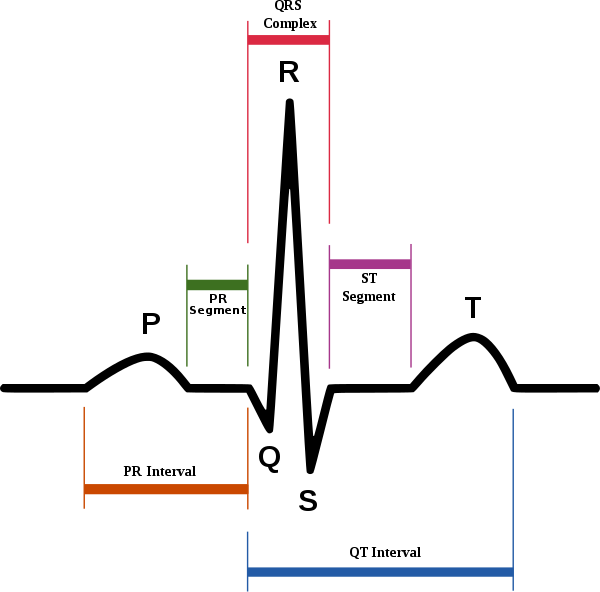
\includegraphics[width=18.5pc]{Definitions/ecgNormal.png}}
%{Images/ecg.png}}
%\widefigure
%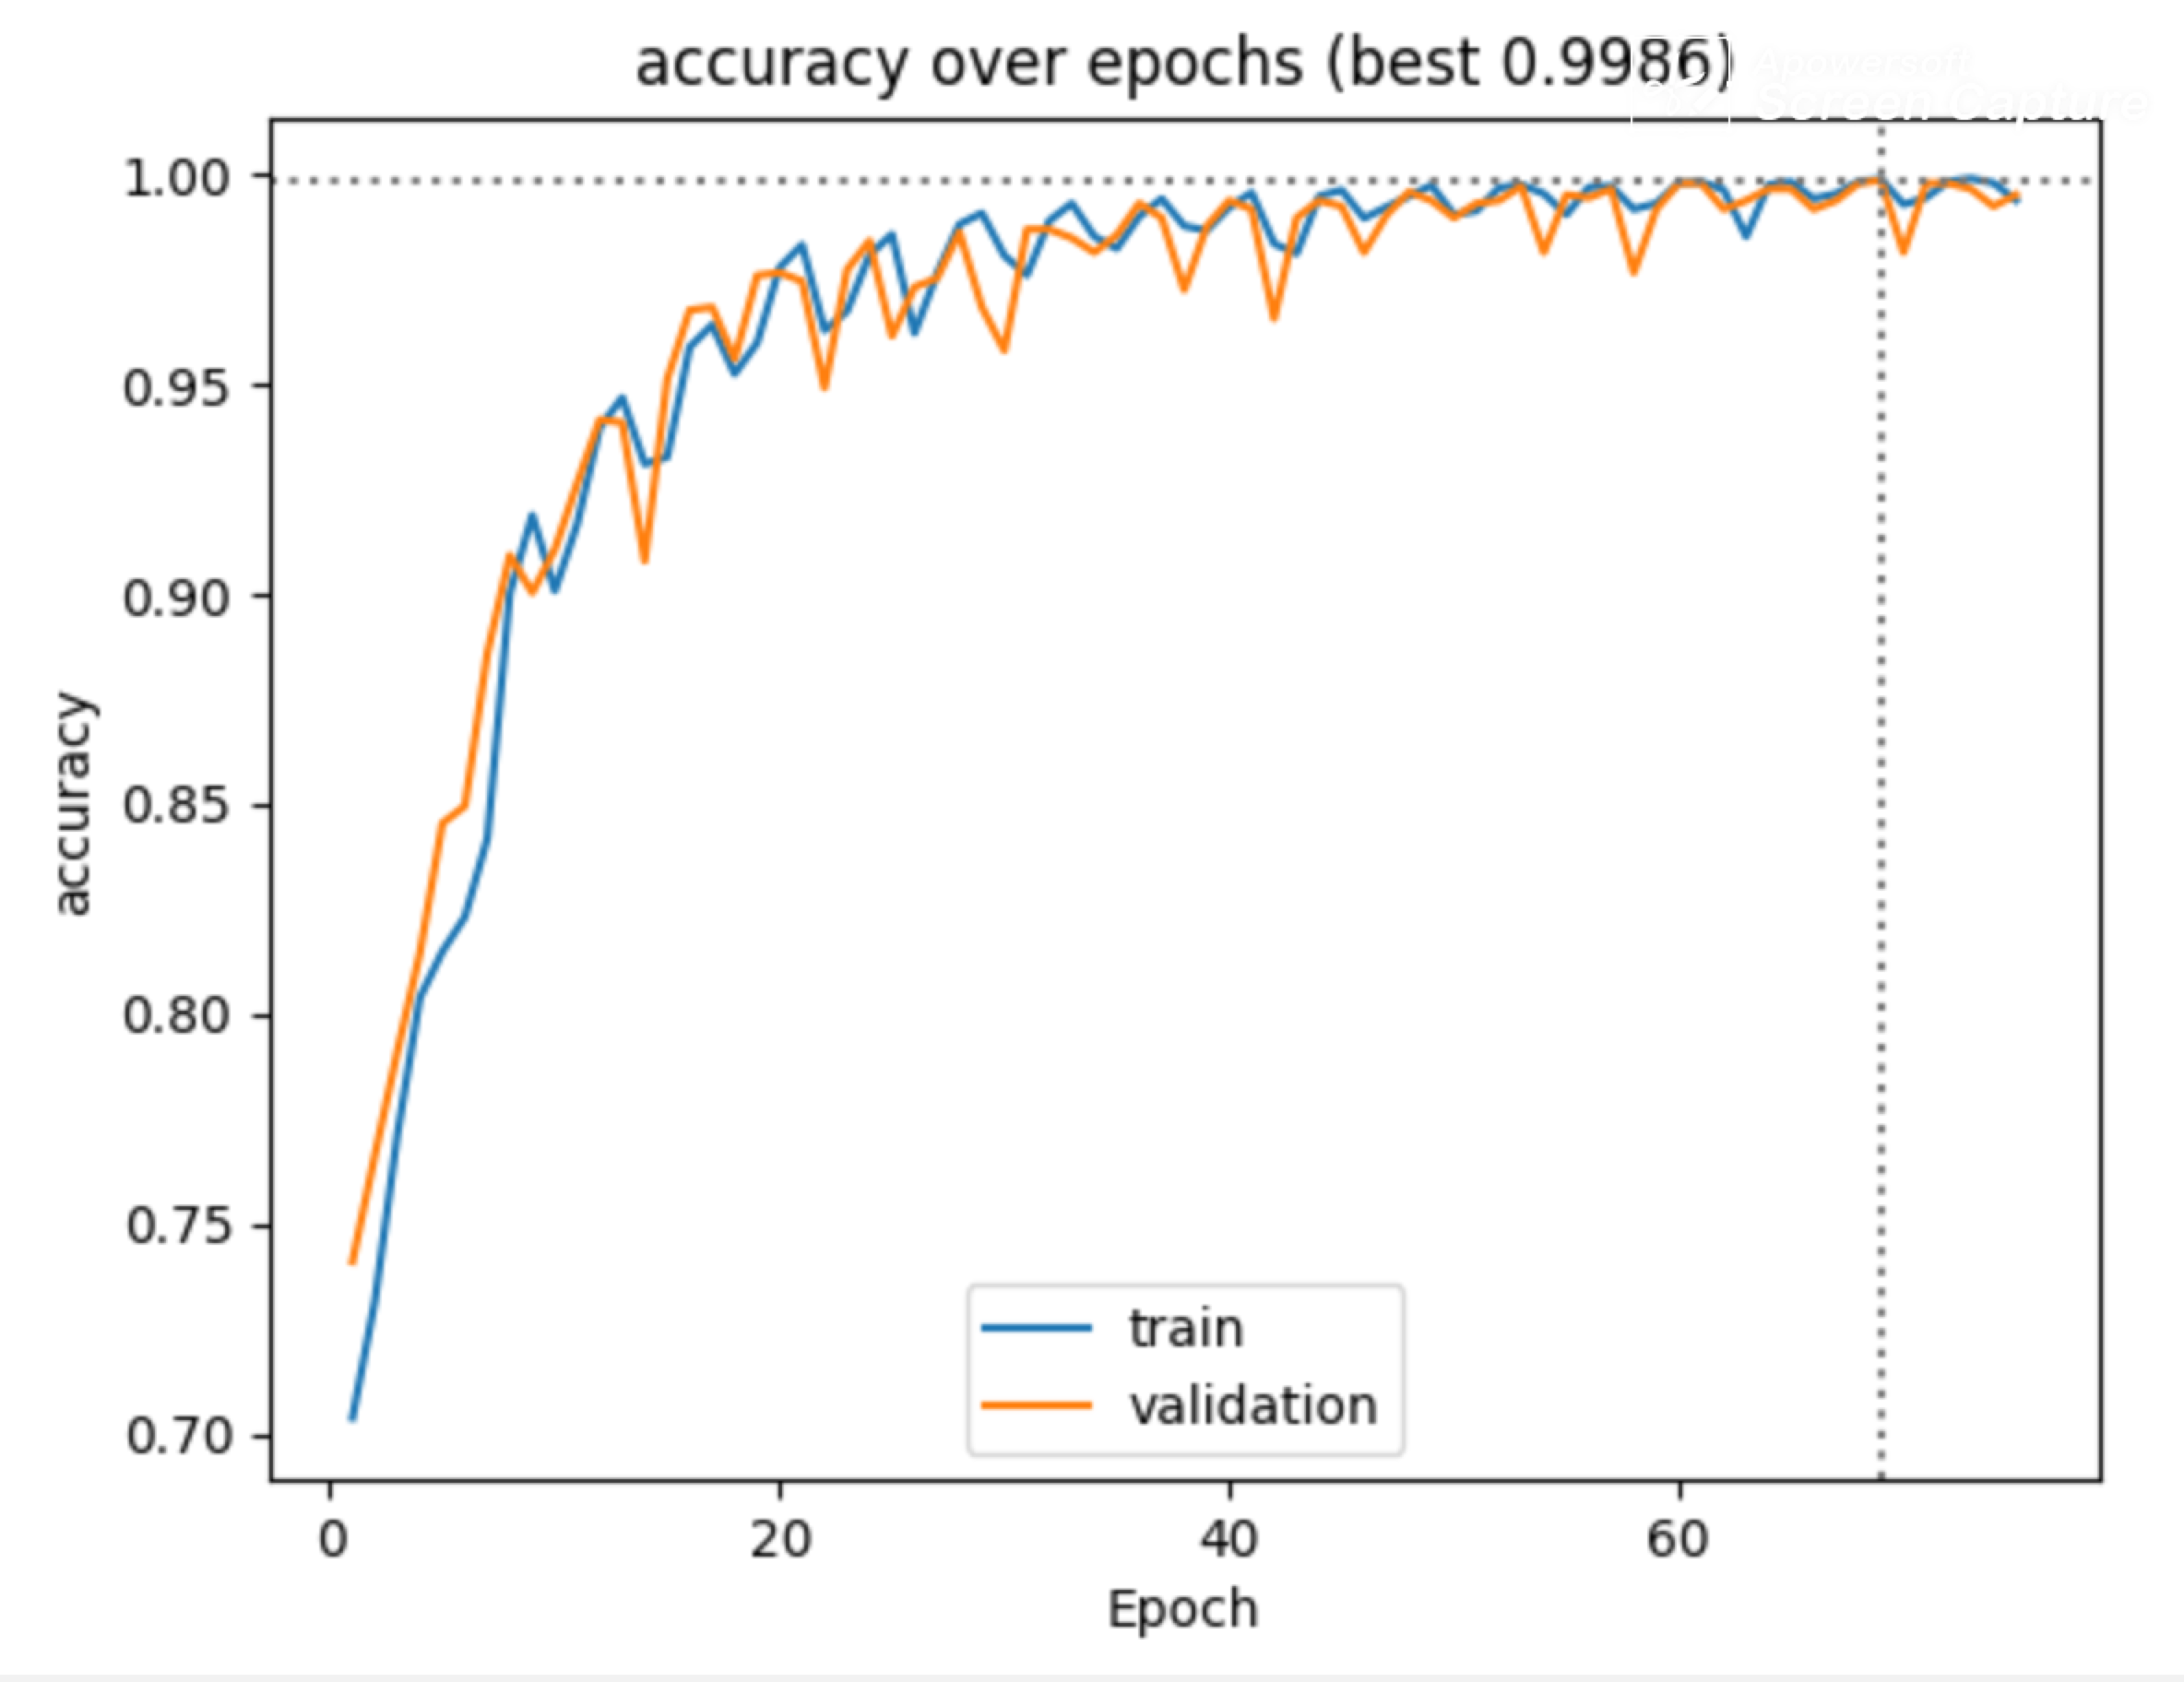
\includegraphics[width=15 cm]{Definitions/PTB_training.png}
%\todo{must check copyright}
\end{figure}


A disruption of blood flow to the muscle layer of the heart causes a cardiovascular condition called a myocardial infarction (MI). This disruption is mostly due to the build-up of the plaques in the arteries which result in reduced blood flow to that part of the heart muscle. MI is called a silent heart attack because the patient is not aware of the condition unless they suffer from a heart attack. An early diagnosis of MI is therefore of vital importance as it would help the patients to get timely treatment hence preventing the high percentage of mortality associated with it. 
Due to the small amplitude (millivolts), the manual interpretation of ECG signals is time-consuming and prone to errors. This limitation can be mitigated by an automatic diagnosis of heart conditions based on the signals. Our study aims to work towards automation of the cardiovascular disease diagnosis from ECG signals.

In this study, we propose two methods to extract features from a time series automatically and then feed those features to another deep learning model for classification.
First, a hybrid model for multiple ECG classification tasks is proposed as an alternative to many complex models which require many pre-processing steps before the actual training. We experimented with a robust hybrid deep learning model for the ECG classification tasks which proved to outperform many state-of-the-art complex models and achieve similar or even better accuracy with no pre-processing steps. The CNN placed in front of a LSTM also known as CNN-LSTM has lately been used for multiple classification tasks but its use for ECG classification has not been systematically explored. The CNN model first searches for the features in high dimensional input data and then after converting it into one-dimensional data, it is fed as an input to LSTM model. The role of the CNN in this context is as an automatic feature extractor.
Secondly, a novel attention/transformer model using wavelets for dimensional embedding is introduced to improve the efficiency of the classification process. As it has less trainable parameters than CNN-LSTM it has advantages in terms of (training) performance as shown in Table~\ref{tbl:attvscnnlstm}. As a bonus, we evaluate both models also on data for fall detection.

\section{Related Work and Our Contribution}

Many recent works focus on automatic ECG classification. Among several different techniques present for ECG classification, deep learning has gained popularity in recent times. It is mainly due to its automatic feature learning and availability of large public data sets. Many deep learning techniques use feature extraction as an essential pre-processing step before feeding the data to the neural network. 
Most common feature extraction techniques for ECG classification are continuous wavelet transform (CWT), discrete cosine transform (DCT) \cite{article2}, Pan-Tompkins algorithm \cite{7019490} and discrete wavelet transform (DWT) {\cite{article}}. One of the major disadvantages of using wavelet transform as a feature extractor is that the complexity of the process increases with the increase in decomposition level. All feature extraction processes require some domain knowledge in order to efficiently extract relevant features from the data. Therefore, we aim to explore the research question of whether a similar state-of-the art results can be achieved with no pre-processing and with a simpler model architecture in an efficient manner in terms of resources and computation. 
Our contribution to this study is twofold. Firstly we use an ensemble of CNN-LSTM to achieve accuracy equivalent to many complex models, and secondly, to further optimize the automatic feature extraction, we introduce a new embedding technique in the attention/transformer encoder architecture which uses discrete wavelet transform to extract features from the ECG time series and feeds them to the attention mechanism. 
In the following sub-sections, we present the state of the art in the related work and highlight our contributions.

\subsection{CNN-LSTM Architectures}

Jambukia et el (2015) \cite{7164783} present an overview of ECG classification into different types of arrhythmia. Another current review on deep learning methods for ECG arrhythmia classification \cite{EBRAHIMI2020100033} deduced that among many deep learning models, CNNs and LSTMs were among the most effective for learning arrhythmia in ECG classification tasks.
The use of CNN-LSTM architecture for classification is not entirely novel. Socher et al. \cite{NIPS2012_3eae62bb} in 2012 proposed a model for 3d object classification which combined a CNN with an RNN. They concluded that the CNN provides the translation variance for lower level features whereas RNNs can learn the interactions and compositional features in the data. Zheng et al \cite{zheng}, transformed the data acquired by three-axis accelerometer into an image format and then used CNN with three convolution layers to classify human activities. XIA et al. (2020), \cite{xia}  used CNN after a LSTM layer to classify human activity recognition (HAR) with an accuracy of 95.85\%. Ordóñez et al.(2016),\cite{ordonez} proposed an activity recognition classifier, which combined deep CNN and dense layers. 
However, not many studies focus on hybrid CNN-LSTM models for ECG classification. Studies like \cite{8419425},\cite{2019},\cite{WANG2021106006} and \cite{e23010119} have implemented CNNs and its variants for ECG classifications. \cite{saadat} used RNNs to classify ECG signals. In this study, we have not only performed multiple classifications with CNN-LSTM model for ECG but also worked with three different ECG data sets including data for fall detection to present proof of concept that CNN placed in front of LSTM surpasses many complex and pre-trained models.

\subsection{Attention and Transformer Architectures}
The seminal paper by Vaswani et al.~``Attention is All you Need" \cite{VaswaniEtAl} has triggered an enormous amount of successful applications of attention mechanisms and transformer architectures in deep learning. however, the vast majority of research is focusing on the natural language processing (NLP) domain. Little research has been carried out in applying attention-based architectures in other domains such as time series analysis. One of the first papers in this regard is LSTNet by Lai et al.~\cite{LaiEtAl}, where the authors introduce long- and short-term time-series network (LSTNet) using the convolution neural networks and  recurrent neural networks to extract short-term local dependency patterns and to discover long-term patterns for time series trends. In \cite{ShunYaoEtAl} Shun-Yao Shih et al.\ apply an attention mechanism for multivariate time series data in three medical domains. Song et al.~\cite{SongEtAl} have applied attention models to clinical time series analysis. A systematic and comprehensive analysis and study of utilising attention mechanisms, however, in the time-series domain is still outstanding.

One of the shortcomings of the self-attention mechanism preventing its application for e.g.\ time-series is the  ${\cal O}(n^2)$ complexity with regards to the length of the input vector, i.e.\ the length of the time series in our case. To address this problem LinFormer has been introduced by Wang et al.\ in \cite{WangEtAl}. Linformer is the first theoretically proven linear-time transformer architecture and henceforth might be suitable also for long time series. The linear scaling is achieved by discovering that self-attention is low rank and henceforth projecting information on a low rank constant sub-dimensions achieves to decouple from the ${\cal O}(n^2)$ scaling. Recently Rabe and Staats \cite{RabeStaats} have proposed an algorithmic solution to at least reduce the memory (but not the time) complexity from  ${\cal O}(n^2)$ to  ${\cal O}(n)$.

In this paper, we propose a novel attention architecture using projection on discrete wavelet components as a means to address the ${\cal O}(n^2)$ problem and for dimensional embedding. Moreover, the results show that using this technique, an \emph{attention only} architecture is on par with or even outperforms more complex models and has several additional advantages such as e.g.\ better run-time performance.


\section{Algorithms}
This section provides a brief overview of the algorithms and the technologies that were used during the course of this study and also presents the state of the art in the respective technologies.

\subsection{CNN-LSTM Model}
We define some basic terms related to the convolutional neural network and LSTM for clarity in the following section.
\subsubsection{CNNs and LSTMs }
Convolutional neural networks, introduced as LeNet in 1989 by LeCunn, have revolutionized the field of image recognition and are among the most prominently used deep neural networks. They were named after the linear matrix operation called convolution. Since convolution is a linear operation, the convolution layer is often followed by a non-linear layer. Though introduced earlier, it gained popularity after its application as the first deep neural network applied for object recognition in ImageNet Large Scale Visual Recognition Competition (ILSVRC) in 2012. AlexNet proved to excel on the largest computer vision data set as compared to contemporary methods. In recent times, \cite{cite-key1} presents a state of the art review of the recent deep CNNs architectures. The individual CNN components are explained in \cite{8308186} in a structured way.
The most common architectures of CNNs include an input layer, a convolution layer followed by a pooling layer, a drop-out layer, and a fully connected layer followed by an output layer. The number of layers and their layout can change depending on different problem sets. The convolution operation\footnote{in the two dimensional case -- the one-dimensional case is analogous} itself is given by:
\begin{align*}
V_{i,j}= X*W_{i,j}+b    &= \sum_{L}X^L*W^L_{i,j}+b \\
                        &=  \sum_{L}\sum_{k,l} X^L_{kl}*W^L_{i+k,j+l}+b
\end{align*}
where $X$ or $X^L$ resp.\ denote the $L$-th input matrix. $W$ is the convolution kernel matrix, $b$ is the bias, and $V_{i,j}$ is the output matrix after convolution. %\cite{zhang}. 

CNNs have been known for thier excellent feature extraction capability. One of the most salient features of CNN is its translation invariance. Therefore, it can extract features irrespective of the spatial context. Though it has proven to be beneficial in image recognition, its application and usefulness in time series is still to be exploited fully. Cases, where historical context is relevant for classification, would not work well with CNN alone as it does not carry any information about the history of the time series. The CNNs initially extract the local features in the sub-regions of the time series and then the information is merged in later stages to detect the higher order features. We applied 1D convolution to the time series both with univariate and multivariate data sets. ECG Human activity recognition (HAR) data set and PTB diagnostic data set contained one feature each, so the 2D convolutional operation would not be suitable as it will incorrectly convolve across multiple time series. 
Long short term memory (LSTM) networks -- a variation of recurrent neural networks (RNNs) -- were introduced by Hochreiter \cite{LSTM} in 1997. They tend to present a solution to the common problem associated with RNNs called vanishing and exploding gradients. Classical RNNs can in principle keep track of long term dependencies in the sequence. However in practice, during the backpropagation phase of training, these long term gradients either vanish or explode due to the successive multiplicative operations. A LSTM consists of a chained loop structure. Each LSTM unit is made up of an input gate, an output gate and a forget gate. The LSTMs keep the long term memory by maintaining a cell state that sustains a part of the information from earlier states by forgetting and/or applying increment operations on the previous states. Adding a CNN in front of a LSTM helps to feed the LSTM the features from CNN which were extracted from the time series.
\subsubsection{CNN-LSTM Architecture and Algorithm}

%Fig.~\ref{fig:CNN-LSTM} depicts the overall architecture of our model;
Fig.~\ref{fig:CNN-LSTM} and Fig.~\ref{fig:cnnlstmArchitecture} provide a more graphical overview of our model. Initially (1*N) time series with N time stamps are convolved with k filters each of size M*1. Later the k feature maps each of size (N-M)+1 time stamps are generated which are passed through a dropout layer followed by the max pooling layer and later fed into the LSTM layer where the encoded extracted features are fed into it from CNN. LSTM unit is followed by a fully connected or Dense layer which applies Softmax as an output function to classify the input time series into one of the output classes.
\begin{figure}[!ht]
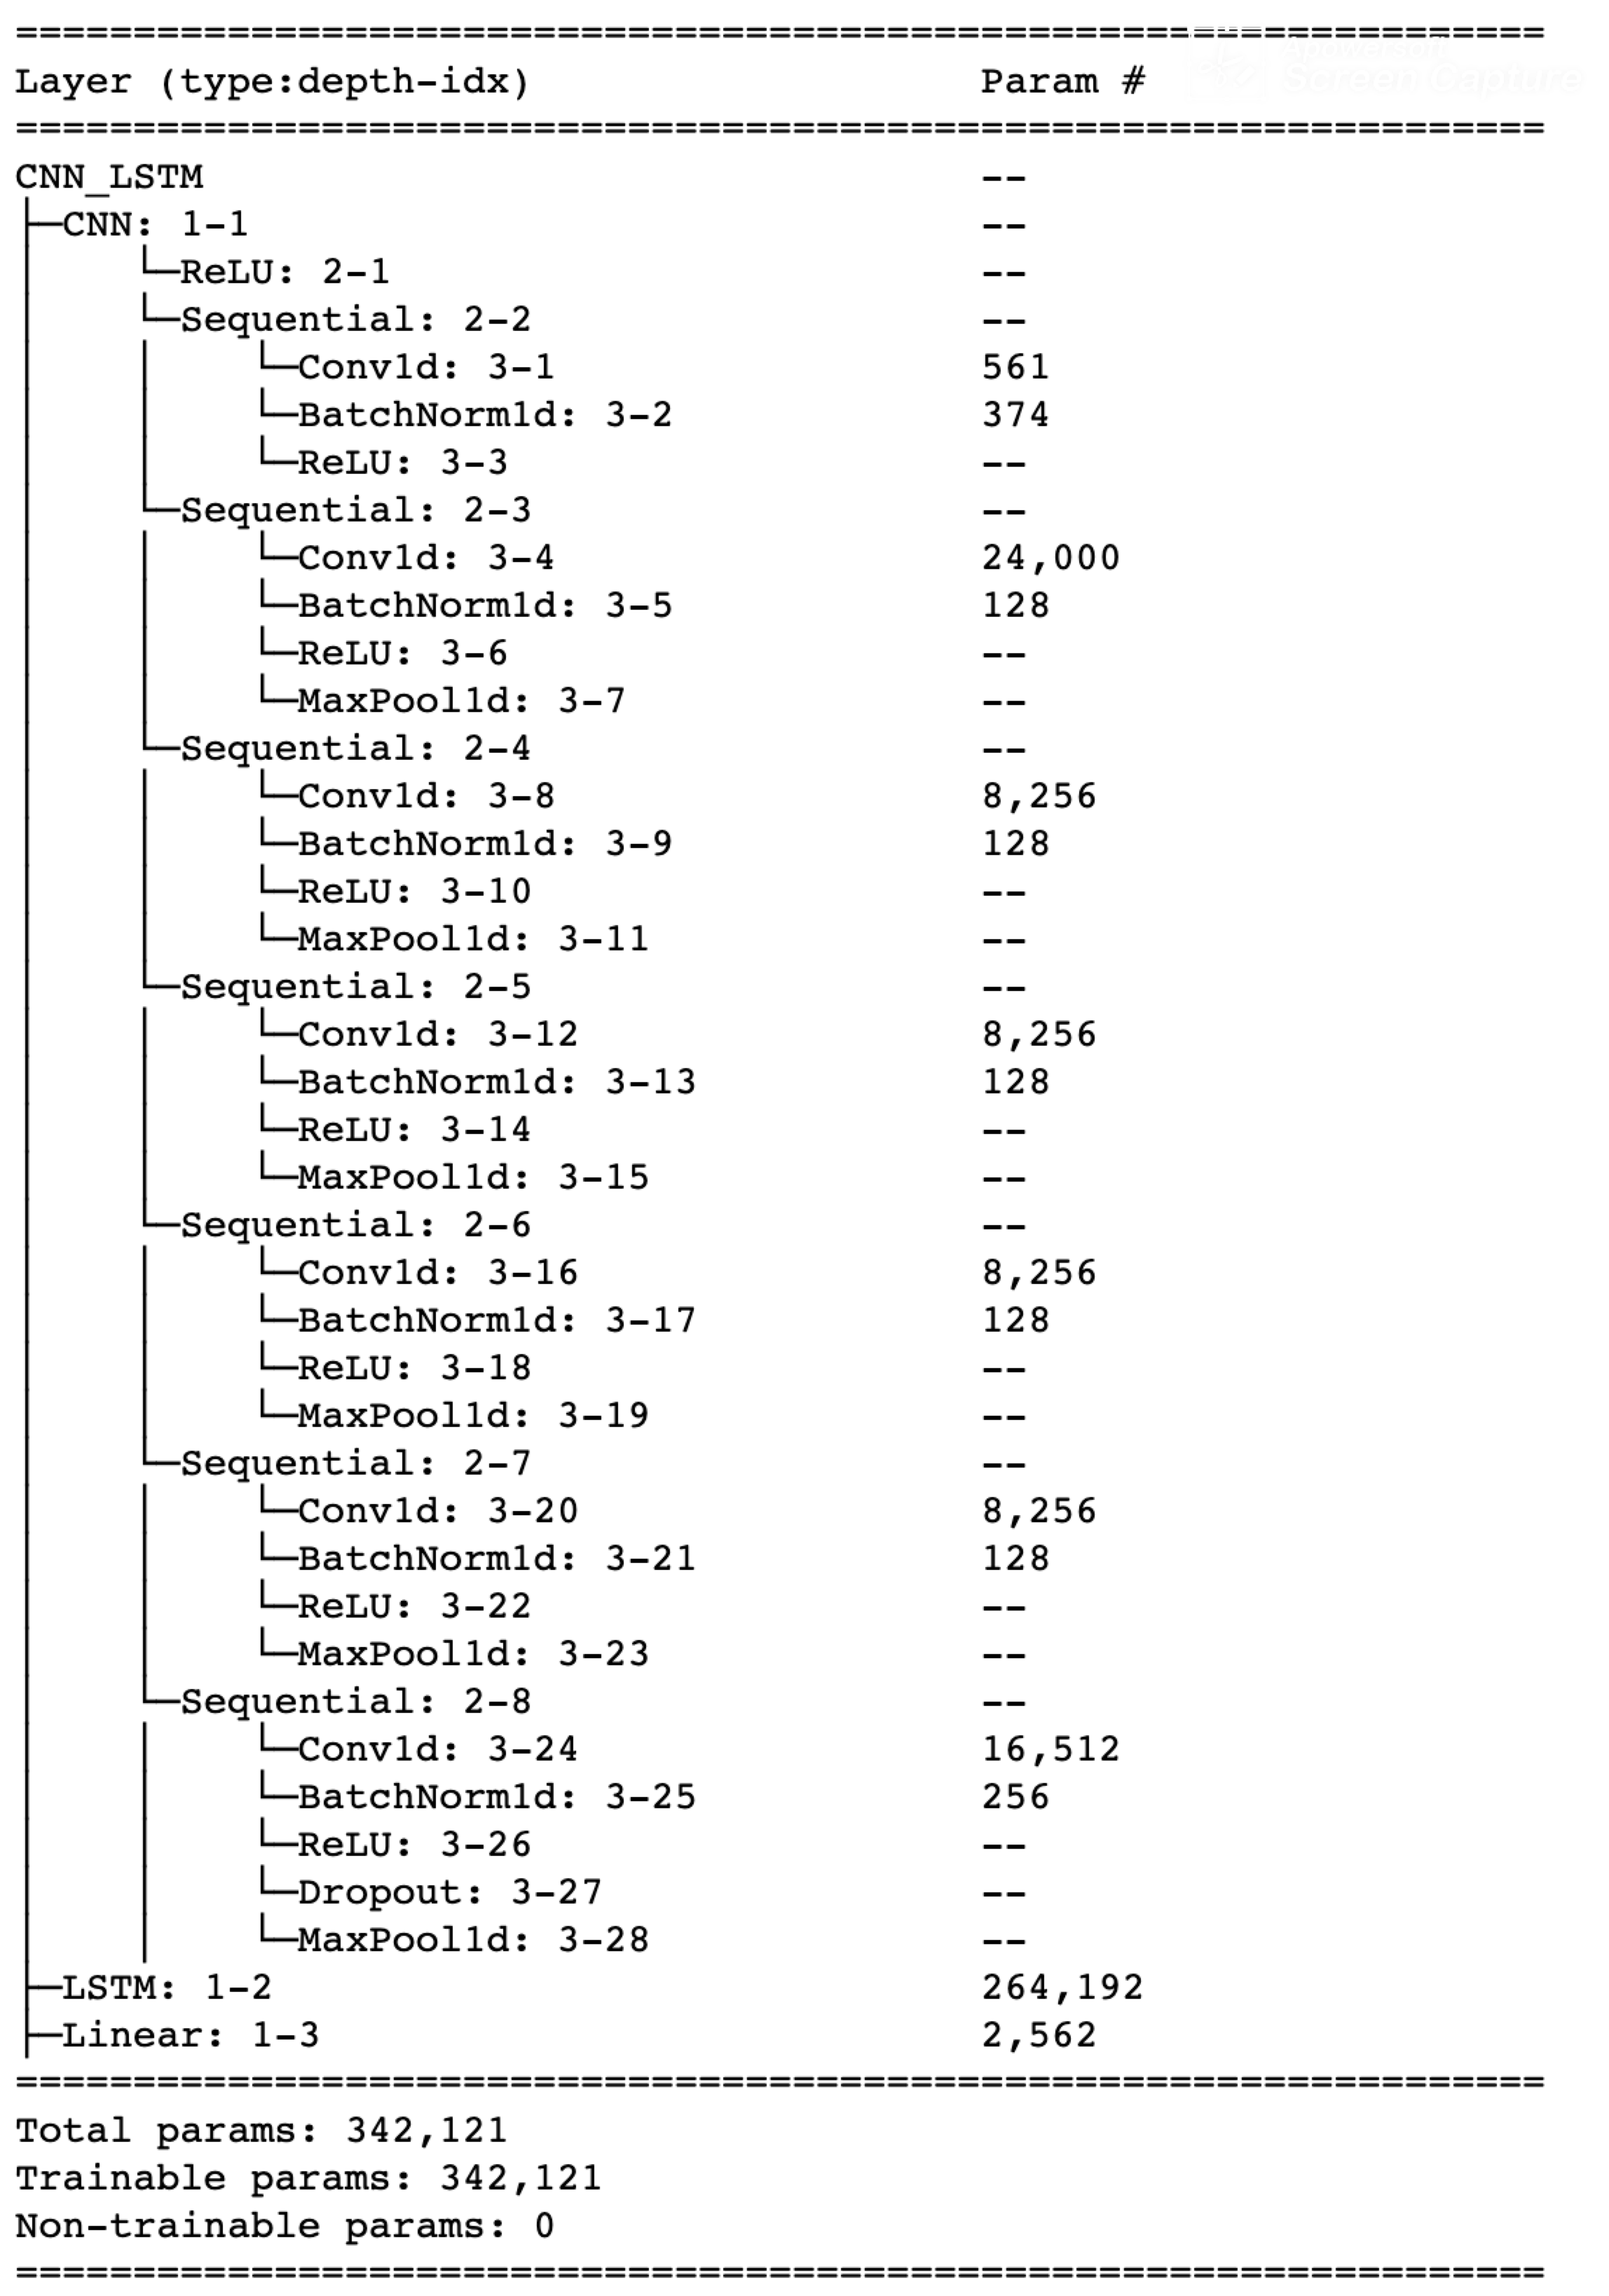
\includegraphics[width=0.5\textwidth]{Images/cnn-lstm.png}
\caption{CNN-LSTM Model for PTB DB}
\label{fig:CNN-LSTM}
\end{figure} 

%\begin{figure}[ht]	
%\centerline{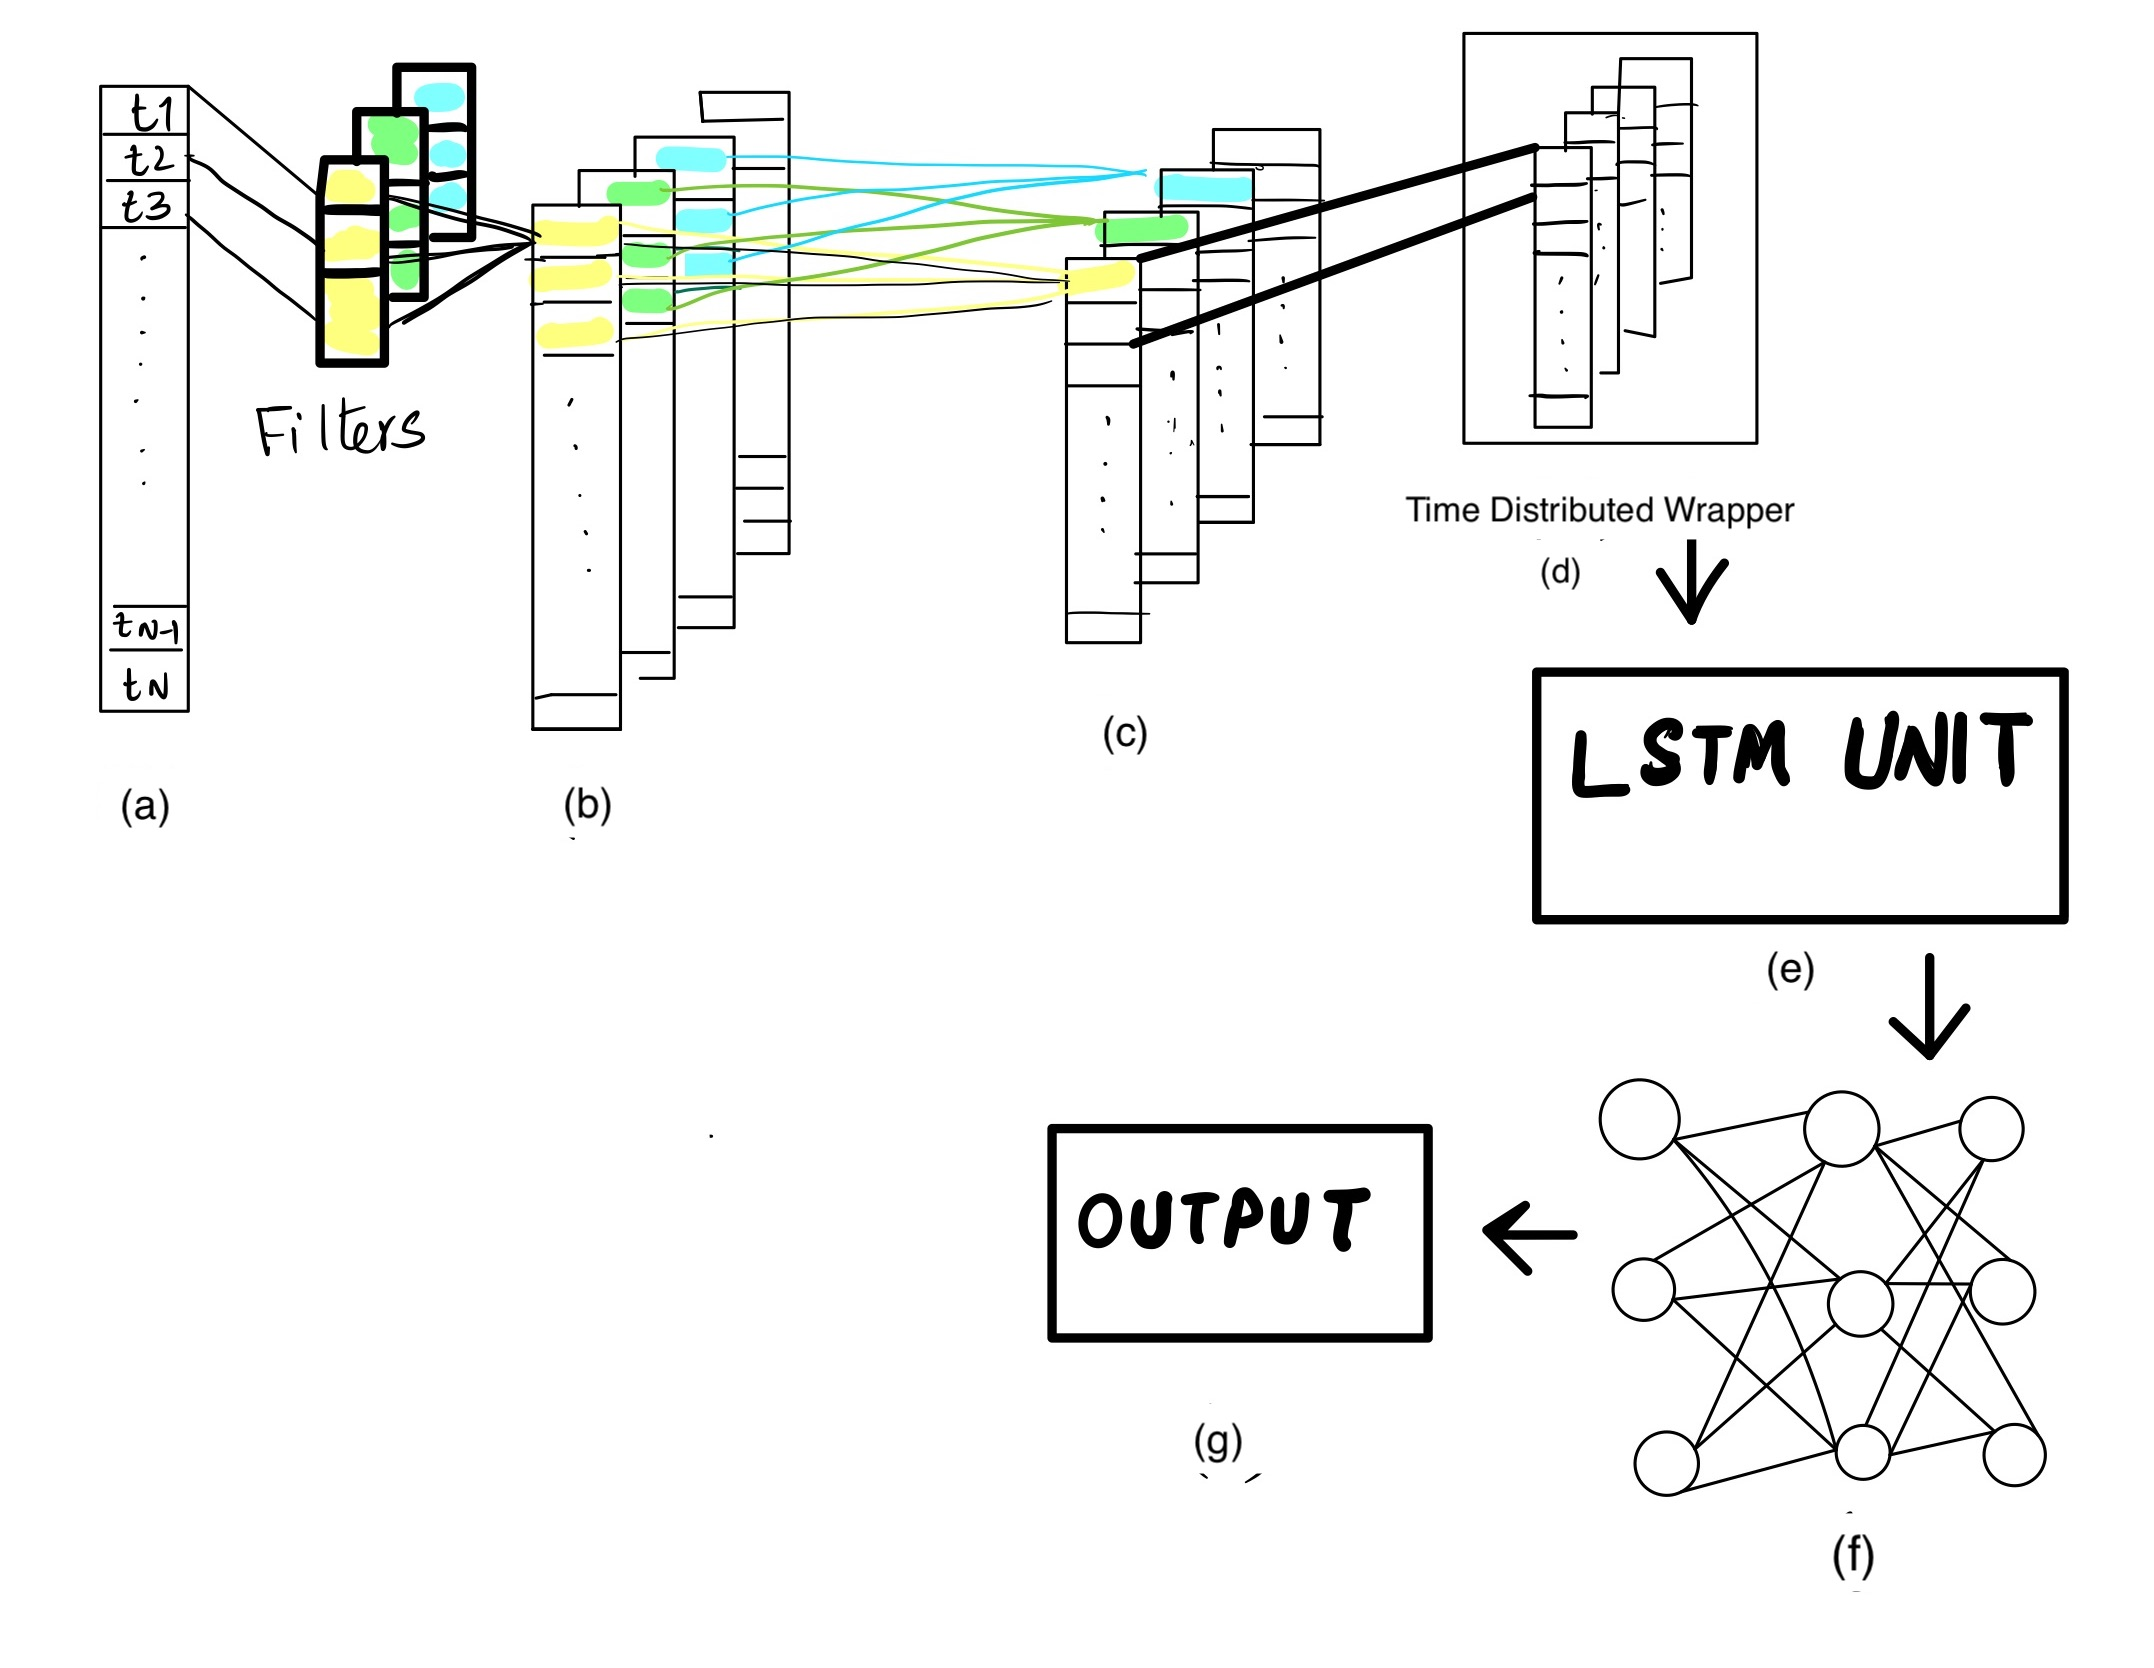
\includegraphics[width=18.5pc]{Definitions/CNN-LSTM.jpg}}
%\caption{A layout of the CNN-LSTM model: (a) A (1*N) time series with N time stamps convolved with k filters each of size M*1, (b) k feature maps each of size (N-M)+1 time stamps, (c)Max pooling followed by (d) dropout and later fed into (e) time distributed layer which feeds the encoded extracted features maps from CNN to (f) LSTM unit. LSTM unit is followed by a fully connected or Dense layer which applies Softmax as an output function to classify the input time series into one of the output classes  \label{fig:CNNModel}}
%\label{fig:CNN-LSTM2}
%\end{figure}

\begin{figure}[ht]
\centerline{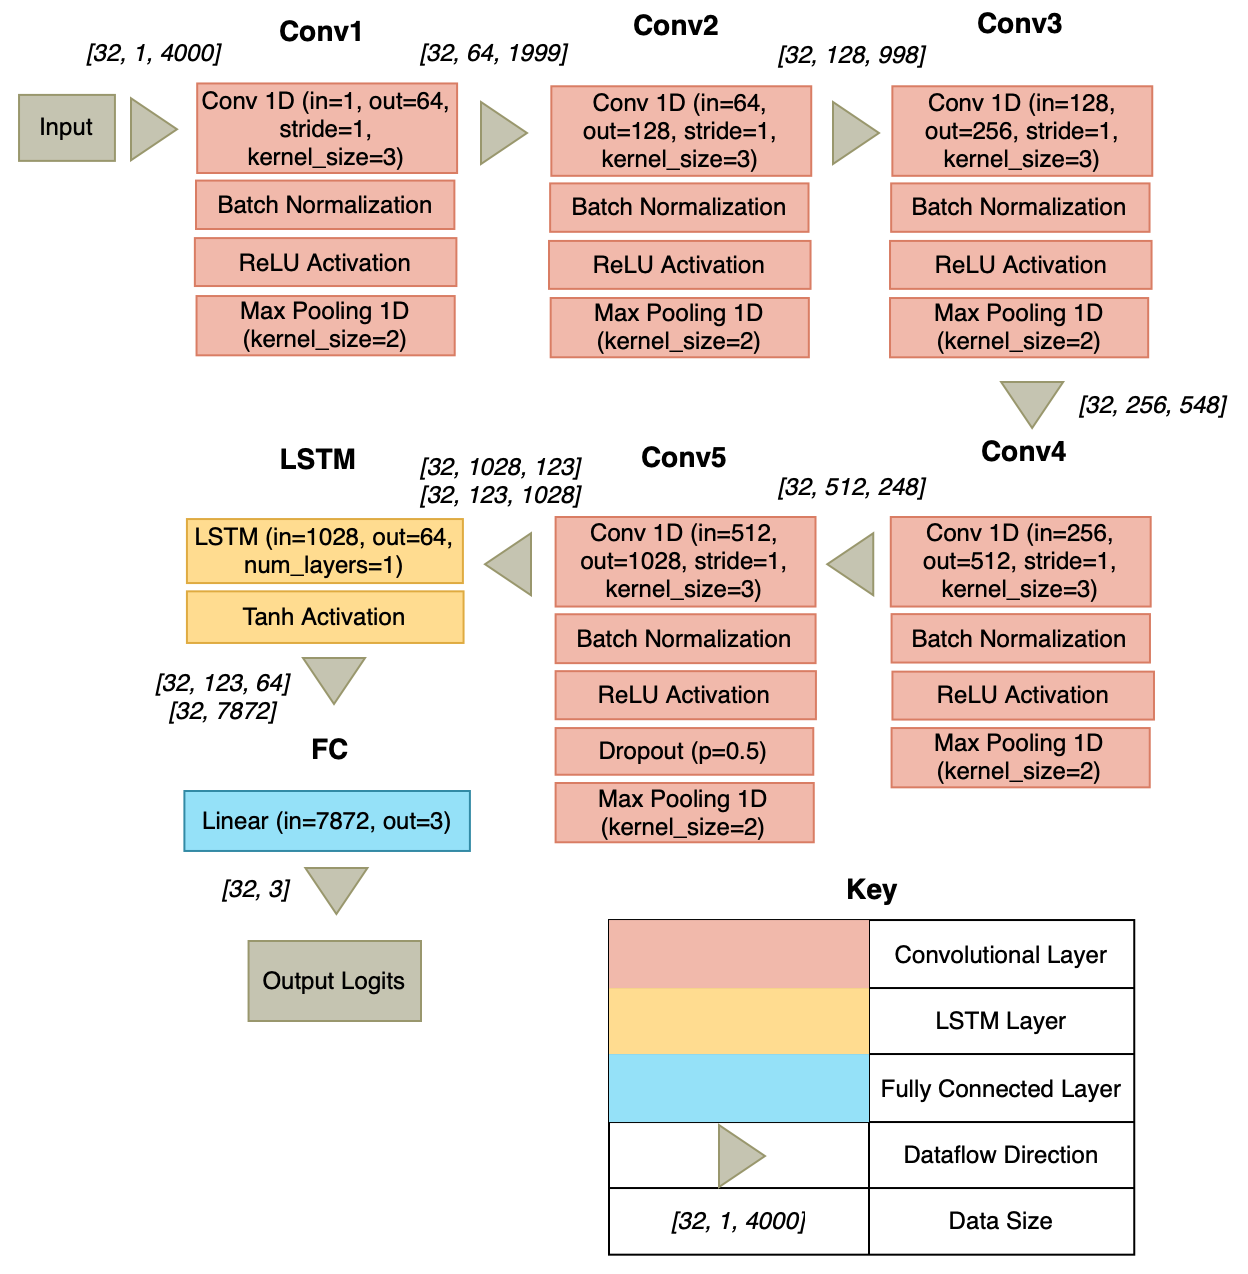
\includegraphics[width=18.5pc]{Definitions/final-cnnlstm-arch.png}}
%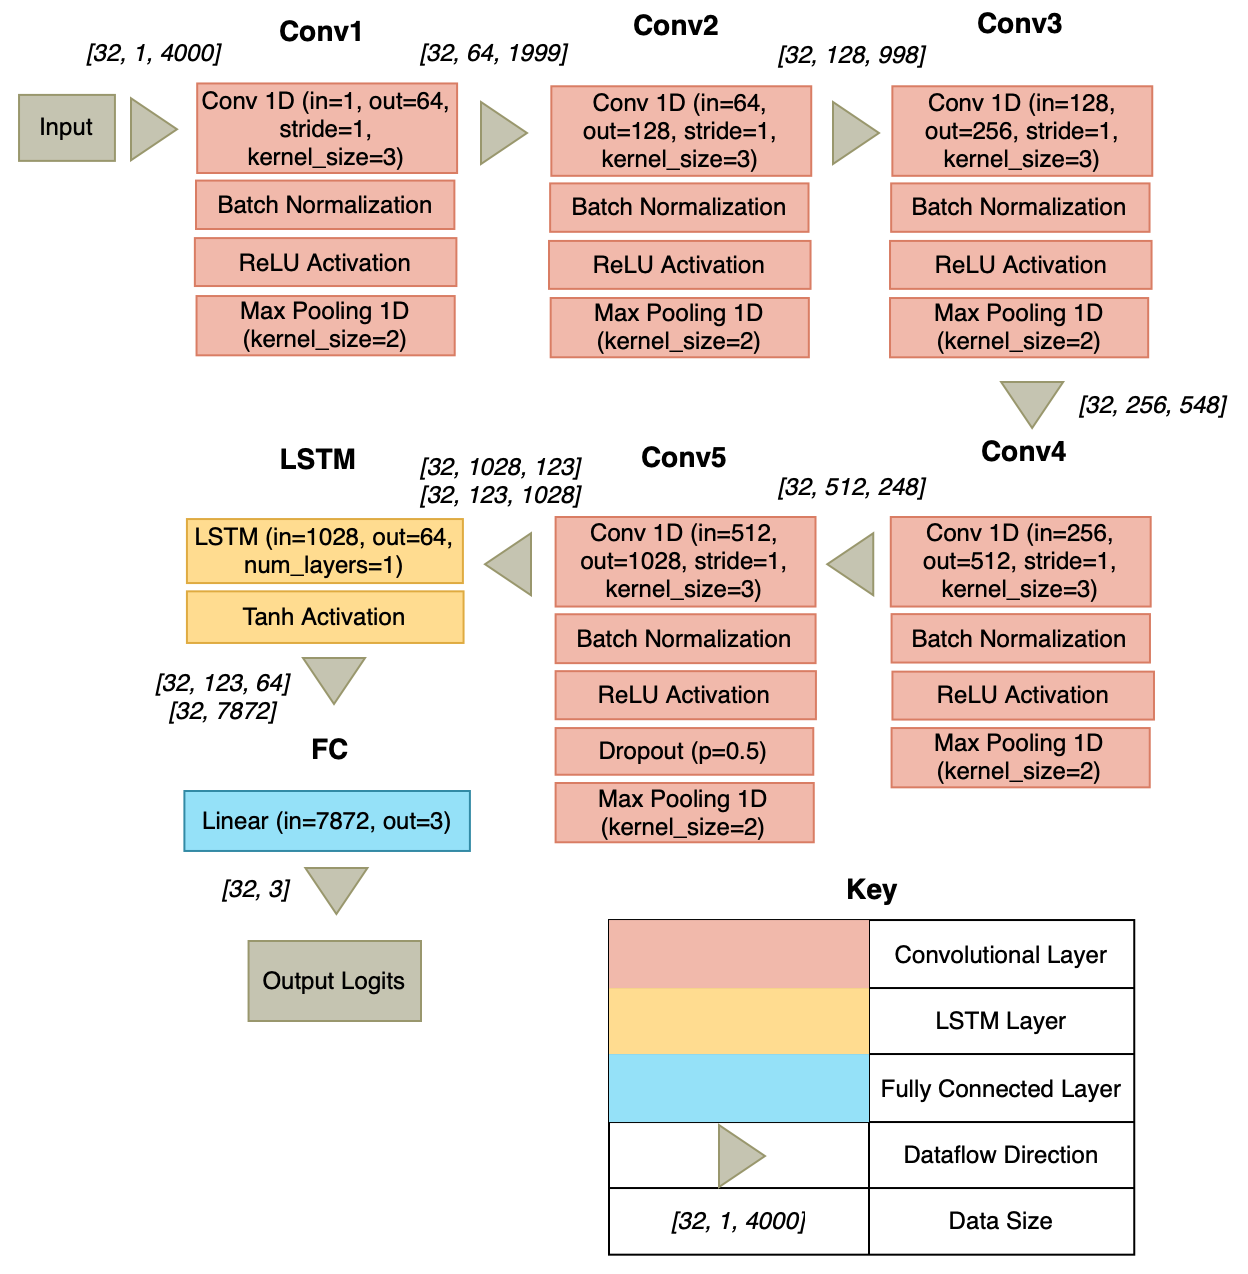
\includegraphics[width=10.5 cm]{Definitions/final-cnnlstm-arch.png}
\caption{Final CNN-LSTM architecture for fall and HAR using ECG signals}
\label{fig:cnnlstmArchitecture}
\end{figure}  




\begin{algorithm}
 \caption{Classification of ECG signals with Raw Signals using CNN-LSTM}
  \label{alg:algorithm1}
 \begin{algorithmic}[1]
 \renewcommand{\algorithmicrequire}{\textbf{Input:} A time series ECG raw data $ts$}
 \renewcommand{\algorithmicensure}{\textbf{Output:} The classified label $l$}
 \REQUIRE 
 \ENSURE  

\STATE $ts \leftarrow$  RAW\_VALUE\_EXTRACTION($ts$)
\STATE $features \leftarrow$ CNN($ts$)
\STATE $l \leftarrow$ LSTM\_CLASSIFICATION($features$)
 \RETURN $l$
\end{algorithmic}
\end{algorithm}
Algorithm \ref{alg:algorithm1} layouts the algorithms for extracting features from the ECG signal and classifying them using a CNN-LSTM model. The number of CNNs and LSTMs can be varied but we used a maximum of 5 1-d convolution layers in front of 3 LSTM layers.
\subsection{Attention Model}
For the reader's convenience, we recall the basic definitions of the attention mechanism following \cite{VaswaniEtAl}.

\subsubsection{Attention}
\newcommand {\softmax}{\mathop{}\,\mathrm{softmax}}

Attention is defined as
\begin{equation}
Attention(Q, K, V)=\softmax \left(\frac{QK^T}{\sqrt{d_k}} \right) V.
\end{equation}

The transformer uses Multi-Head Self-Attention (MHA) allowing the model to jointly attend to information at different positions of the time-series or different semantics of the domain. MHA is defined as 
\begin{align} 
&\text{MultiHead}(Q, K, V) = \\
&\text{Concat}\left(\text{head}_1, \text{head}_2, \ldots, \text{head}_h \right)  W^O, 
\end{align} 


where $Q$, $K$ and $V\in \mathbb{R}^{n\times d_m}$ are input embedding matrices, $n$ is the length of the (time) series, and $d_m$ is the embedding dimensions, and $h$ is the number of heads. Each head is defined as

\begin{align} 
\text{head}_i 	&= \text{Attention}(QW_i^Q, KW_i^K, VW_i^V) \\
			&= \softmax \left[\frac{QW_i^Q(KW_i^K)^T}{\sqrt{d_k}} \right] VW_i^V,
\end{align} 
where $W_i^Q$, $W_i^K \in \mathbb{R}^{d_m\times d_k}$, $W_i^V \in \mathbb{R}^{d_m\times d_v}$, and $W^O \in \mathbb{R}^{hd_v\times d_m}$ (projection onto the output) are learned matrices and $d_k$, $d_v$ are hidden dimensions of projection subspaces. For simplicity in the sequel, we drop the differentiation between $d_m$, $d_k$ and $d_v$ and refer to them by $d$. 

The matrices $Q$, $K$ and $V$ are usually referred to as query, key and value matrices to remind of the associative memory architecture of a transform, compare e.g.\ also the analysis in \cite{RamsauerEtAl}.

\subsubsection{Attention and Dimensional Embedding}
For applying the attention mechanism to time-series one has to decide on the proper dimensional embedding, i.e.\ on the dimension of the embedding subspace and on the embedding transformation. We recall that in the domain of ECG the ``natural'' dimension is small. For instance, the signals are one-dimensional if a one-dimensional channel is used (as is the case in this paper for the attention/transformer model, i.e.\ Algorithm~\ref{alg:algorithm2}). Even if multi-channel ECGs are used usually the number of channels is limited to a small number of 3 to maximally 12 channels. Henceforth, if we used the channel as the embedding, the dimension would be $1$ in our case, i.e.\ $d=1$. This is way too small to capture interesting patterns and, indeed, a test showed that the gradient descent does not converge, but stays constant after one or two initial updates. Furthermore, as depicted in the previous section, the self-attention suffers from an  ${\cal O}(n^2)$ problem. We propose the following architecture to solve both problems simultaneously:
\begin{enumerate}
\item Assuming $m \ll n$. For simplicity of the notation, we assume without loss of generality that $n$ is divisible by $m$, i.e.\ $n = mw$. This effectively segments the time-series $n$ into $n_m$  ``windowed'' segments of length $w$, where $m\in 1, \ldots k$ with $k:=n/w$. If $n$ is not divisible without remainder we could fill the time series with zeros (padding).
\item For each ``windowed'' sub- time-series $t_{n_k}$ we calculate the decomposition to a chosen (fixed) wavelet by performing a discrete wavelet transformation (DWT), see below. Assuming that the result of applying the DWT is in dimension $p$, we have transformed the input from $\mathbb{R}^{n}$ into $\mathbb{R}^{m\times p}$ depicted in Fig.~\ref{fig:dimEmbedding}.
\end{enumerate}

\begin{figure}[!ht]
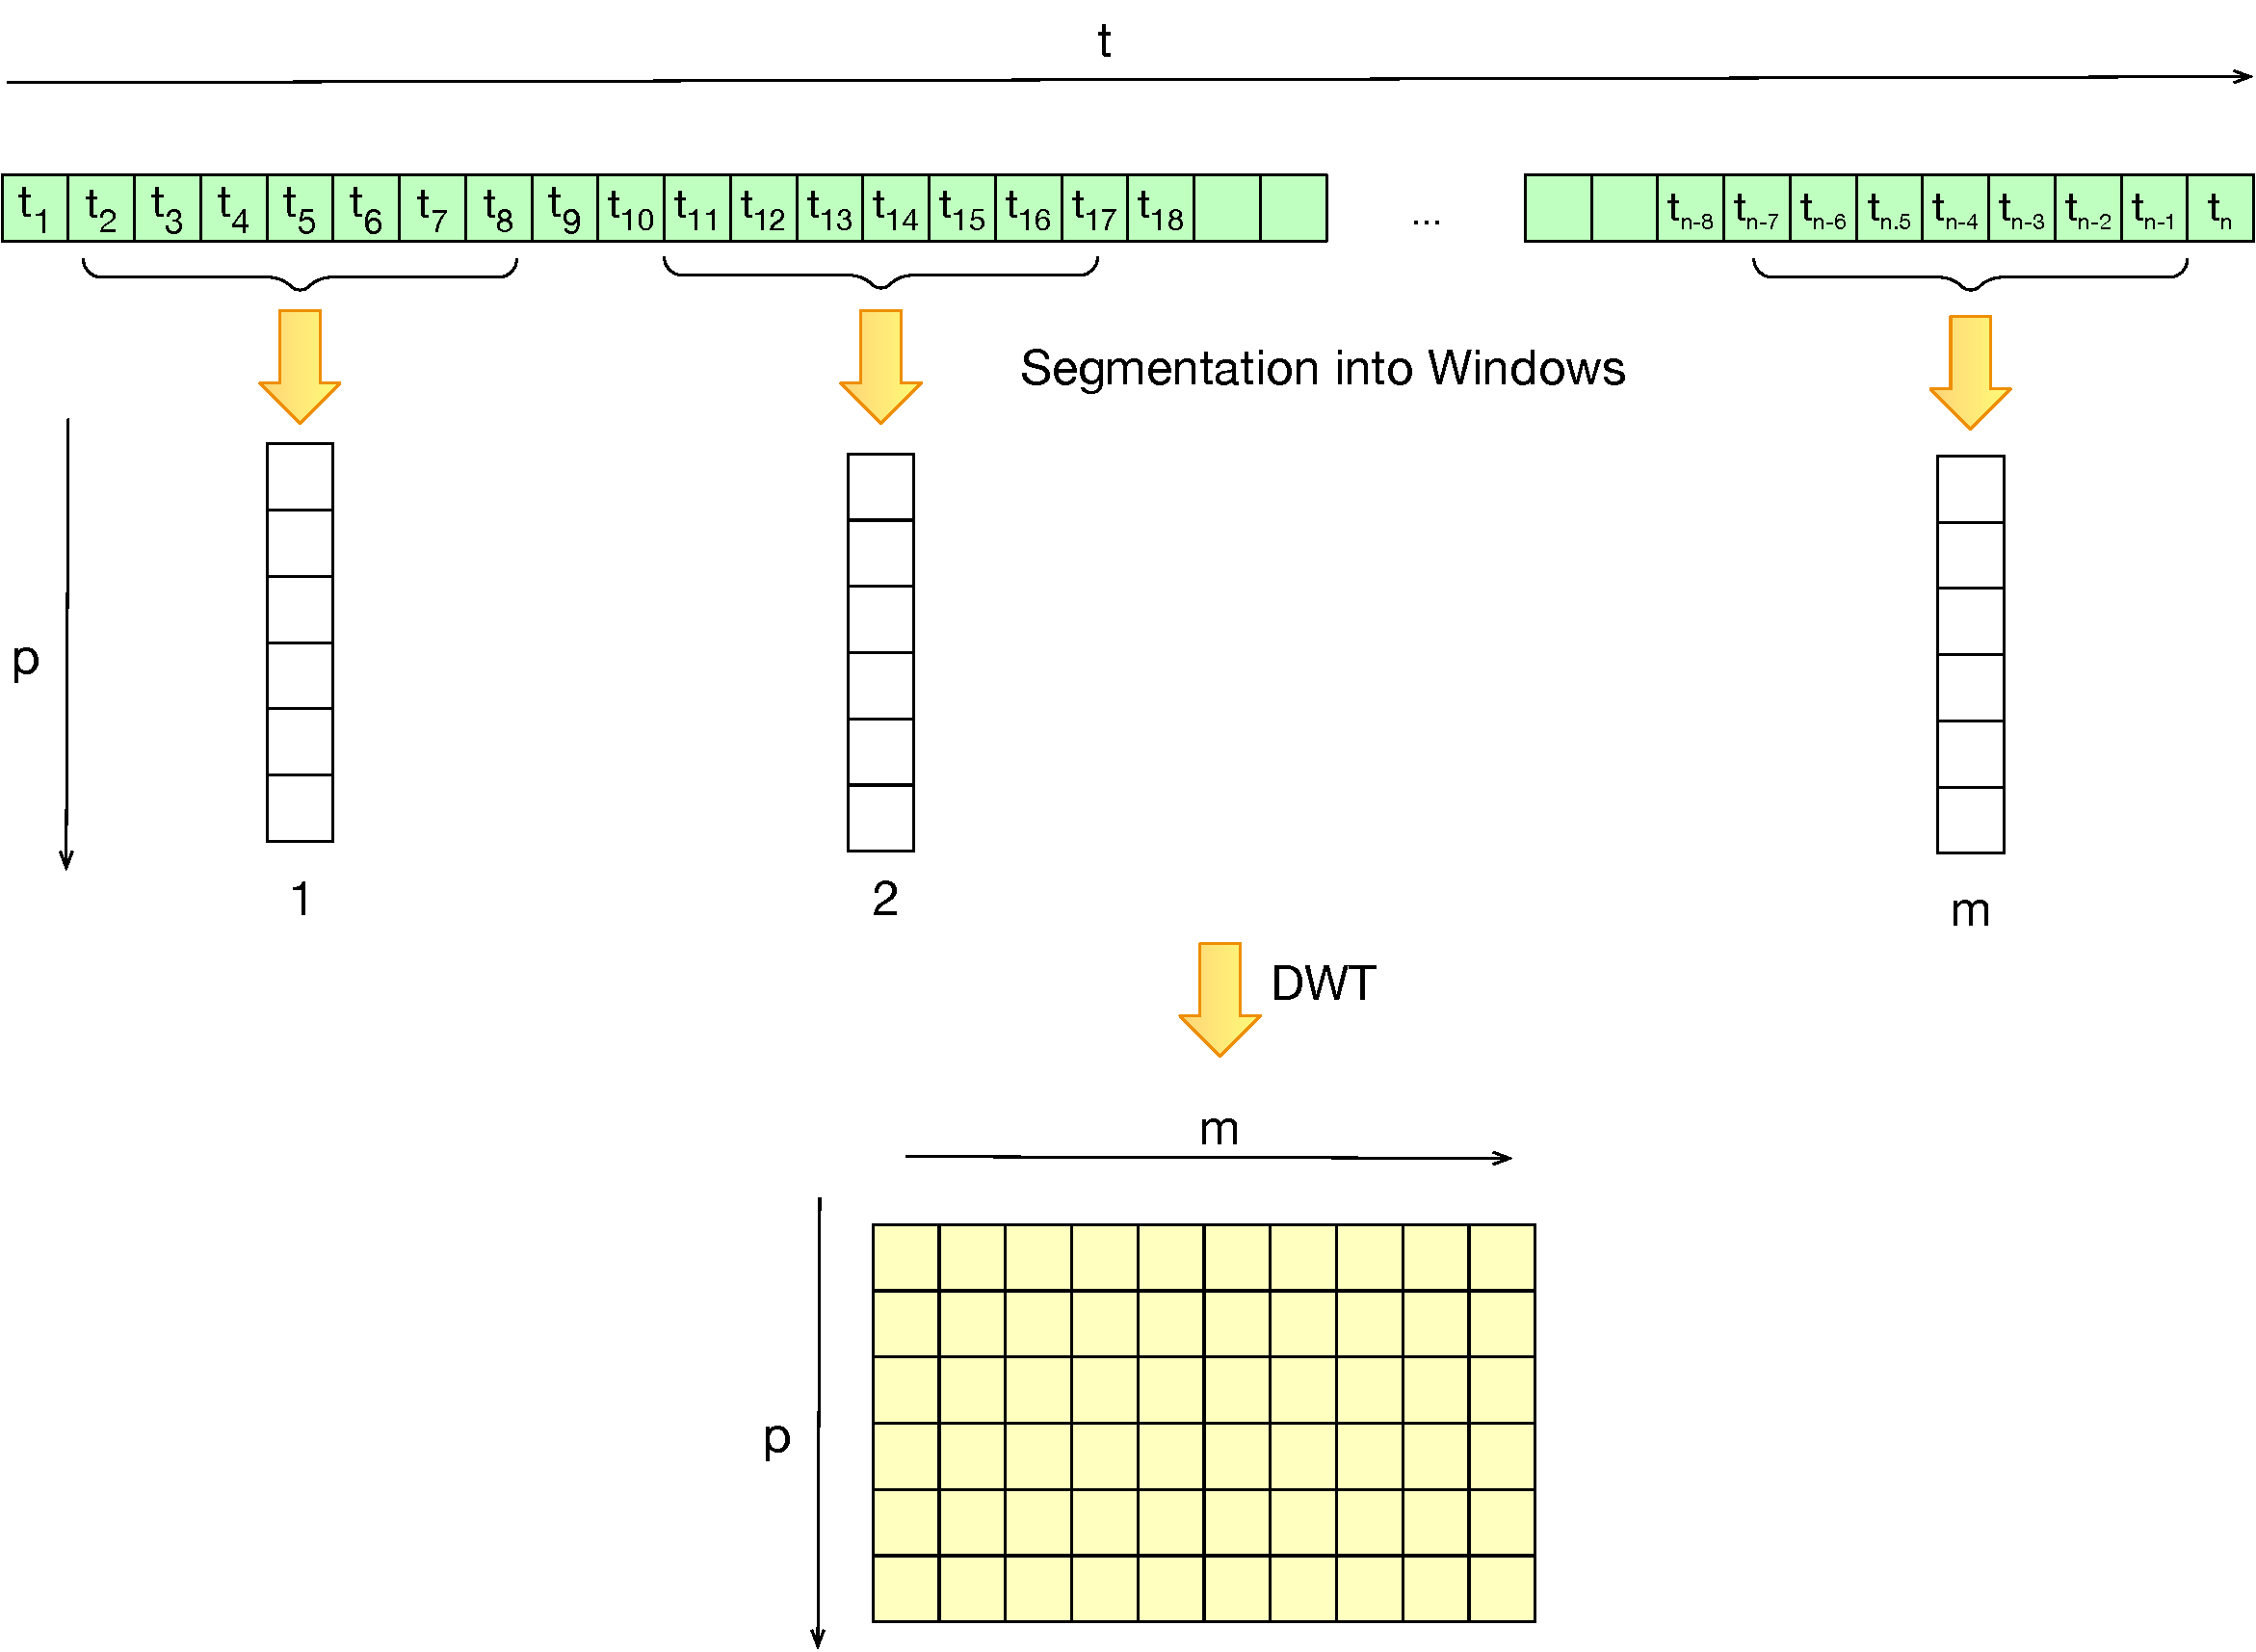
\includegraphics[width=0.5\textwidth]{Images/DimEmbedding}
\caption{Dimensional Embedding\label{fig:dimEmbedding}}
\end{figure}   

\begin{remark} In this paper, we propose a deterministic embedding using DWT rather than a learned, randomly initialised embedding, which is an alternative approach that has been used in other attention architectures in the past. This should -- in theory -- require less training data -- a conjecture that we want to validate in future work using synthesized data.
\end{remark} 

\subsubsection{Discrete Wavelet Transformation (DWT) for Dimensional Embedding}
For the reader's convenience, we recall a few well-known definitions and theorems wavelet theory following \cite{Daubechies} and \cite{MallatEtAl}.
%\todo{Look into the notation of mother wavelet with t as denominator - done and confirmed, but added the details such as integration constant to make more obvious. Note, that the admissibility condition implies \psi(0)=0 as it should be}
We consider signals as real-valued functions. We call a function $\psi\in L^2(\mathbb{R})$ an orthonormal wavelet ifs dyadic translations and dilations of $\psi _{{jk}}(x)=2^{{\frac  {j}{2}}}\psi \left(2^{j}x-k\right)$ constitute a Hilbert space and if in addition, it satisfies a regularity (admissibility) condition, namely $\int_0^\infty |\psi(t)|^2 \frac{dt}{t}<\infty$, ensuring convergence and $\int \psi(t)\, dt =0$. The function  $\psi$ is usually called the \emph{mother wavelet} and its child wavelets are defined as 
$\psi_{j,k}(t)= \frac{1}{\sqrt{2^j}} \psi \left( \frac{t - k 2^j}{2^j} \right)$. A projection of a function $x(t)$ onto $\psi_{j,k}$ is then given by
\begin{equation}
 \gamma_{jk} = \int_{-\infty}^{\infty} x(t)  \frac{1}{\sqrt{2^j}} \psi \left( \frac{t - k 2^j}{2^j} \right) dt.
\end{equation}
The crucial idea is to decompose the space $L^2(\mathbb{R})$ into resolution spaces of different resolutions. First, the \emph{resolution space} $V_0$ is defined as the space of piecewise constant functions on subintervals of $[n, n+1]$ with $n=0,\ldots, N$. if we define the corresponding step function  

\begin{equation}
\phi(t)=\begin{cases}
1, & if\quad  0\leq t<1 \\
0 & otherwise,
\end{cases}
\end{equation}
%
then $V=$ has dimension $N$ and the $N$ functions $\boldsymbol\phi_0 := \{\phi (t-j)\}_{j=0,\ldots, N-1} $ constitute an orthogonal basis. Analogously the \emph{refined resolution spaces} $V_k$ are defined as the spaces of functions constant on each subinterval $[n/2^k, (n+1)/2^k]$. This yields a nested sequence of embedded spaces
\begin{equation}
V_0 \subset V_1 \subset V_2 \subset \ldots \subset V_k.
\label{eq:waveletDecomposition}
\end{equation}
We denote the orthogonal complements of $V_{k-1}$ in $V_k$ as $W_{k-1}$, i.e.\ $V_k= V_{k-1}\oplus W_{k-1}$ and call it the \emph{detail space}. This yields an orthogonal decomposition at level $k$ as follows:
\begin{equation}
V_k = V_0\oplus W_0 \oplus W_1 \oplus \ldots \oplus W_{k-1}
\end{equation} 

Then the $k$-level \emph{discrete wavelet transformation} (DWT) is defined as the change of coordinates from $\boldsymbol\phi_k$ to $(\boldsymbol\phi_0, \boldsymbol\psi_0, \boldsymbol\psi_1, \ldots, \boldsymbol\psi_{k-1}$), where $\boldsymbol\phi_k := \{\phi_{jk}\}_{j=0,\ldots, N-1}$ and $\boldsymbol\psi_k := \{\psi_{jk}\}_{j=0,\ldots, N-1}$, resp. denote the family of functions obtained from the mother wavelet.

This yields a filter bank interpretation of DWT, wherein each step the signal is decomposed into an averaged and a detailed signal using low-pass and a high-pass filter depicted graphically in Fig.~\ref{fig:waveletTransformPyramid}.
\begin{figure}[ht]
	\centering
	\diags{1.5em}{0.5em}{
	V_m\ar[r]\ar[ddr]	&V_{m-1}\ar[r]\ar[ddr]&\ldots\ar[r] 	&V_{2}\ar[r] \ar[ddr]	&V_{1}\ar[r] \ar[ddr]	&V_0\cr
					&\oplus			&\oplus		&\oplus			&\oplus			&\oplus\cr
					&W_{m-1}			&W_{m-2}		& \ldots			&W_{1}			&W_0\cr
}
	\caption{Wavelet Transform Pyramid}
	\label{fig:waveletTransformPyramid}
\end{figure}

Thus, any signal can be decomposed into an averaged and a detailed signal, namely $V_0$ and $W_0$. Due to the recursive nature, this can be extended to any desired level $k$. Please note, that due to the dyadic nature the data size is reduced by a factor of $2$ in each step. For further details, we refer to \cite{Daubechies} and \cite{{MallatEtAl}} as well as e.g.\ \cite{Ryan}. 

We used Haar and Daubechies wavelets as well as symlets (symmetrized version of Daubechies wavelets) as a mother wavelet. 

\subsubsection{Transformer Architecture and Algorithm}
The DWT can be used not only for dimensional embedding but also for noise reduction as one can ignore some or all coefficients for the detailed spaces. To explore the impact we tried several configurations, see Table~\ref{tbl:atttentionModels}\footnote{Frequency refers to the frequency of the positional encoding. It should be remarked, that model \textsc{att5} differs from \textsc{att4} by an additional residual connection.}. 

\begin{table}[!ht]
\caption{Attention Models}
\label{tbl:atttentionModels}
\centering
\scriptsize
{%
\renewcommand{\arraystretch}{1.2}
\begin{tabular}{cccccccc}
		&{\rotatebox[origin=l]{90}{Wavelet}}&{\rotatebox[origin=l]{90}{Spaces}}&{\rotatebox[origin=l]{90}{Dim Embedding}}&{\rotatebox[origin=l]{90}{Hid Dim}}&{\rotatebox[origin=l]{90}{Frequency}}&{\rotatebox[origin=l]{90}{Epochs}}&{\rotatebox[origin=l]{90}{Accuracy}}\\
\textsc{att2}		&db8 					&$V_0$				    	&13				&150		&0.1k			&1k		&98.14\\
\textsc{att3}		&db8 					&$V_0$				    	&12 			&150		&0.1k			&1k		&98.83\\
\textsc{att4}		&db8					&$V_0\oplus W_0$	    	&24 			&150		&0.1k			&1k		&99.18\\
\textsc{att5}		&db8 					&$V_0\oplus W_0$	    	&24 			&150		&0.1k			&1k		&99.11\\
\textsc{att6}		&db8					&$V_0\oplus W_0$	    	&26 			&250		&0.1k			&1k		&99.45\\
\textsc{att7}		&sym6 					&$V_0\oplus W_0$	    	&22 			&250		&0.1k			&1k		&99.38\\
\textsc{att8}		&db8					&$V_0\oplus W_0$		    &26 			&250		&10k			&1k		&99.59\\
\textsc{att9}		&db8					&$V_0\oplus W_0$	       	&26 			&250		&10k			&2k		&99.59\\
\textsc{att10}		&db5					&$V_0\oplus W_0$	    	&20				&250		&10k			&1k		&99.24\\
\textsc{att11}		&db5 					&$V_0\oplus W_0\oplus W_1$  &28 			&250		&10k			&1k		&99.73\\
\end{tabular}
\medskip	
}
\end{table}

We deployed a transformer architecture with one head, four transformer encoder layers, and a dimension of 150 or 250 hidden units of the feed-forward network. The network's architecture of the best model, \textsc{att11}, is depicted in Fig.~\ref{fig:transformerArchitecture}.
\begin{figure}[!ht]
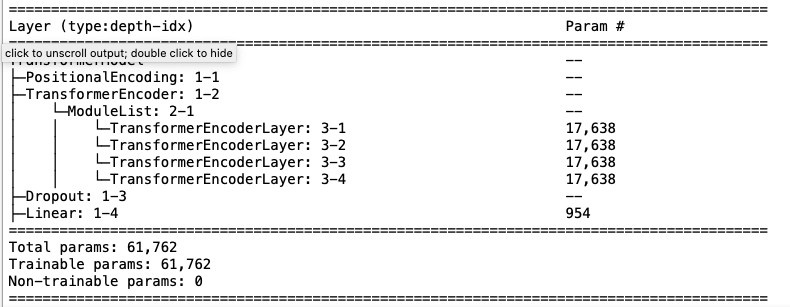
\includegraphics[width=0.5\textwidth]{Images/TransformerArchitecture}
\caption{Transformer Architecture of Model \textsc{att11}}
\label{fig:transformerArchitecture}
\end{figure}   

The original input tensor has a dimension of $[14552, 1, 187]$ corresponding to $14522$ data rows, $1$ feature, and a sequence length of $187$. The sequence was split into $17$ chunks of window length $11$. Each subsequence of length $11$ was converted using DWT. For instance, for db8 for \textsc{att7}, this leads to a transformed tensor of $[14552, 22, 17]$. (Note, that due to boundary effects, the embedding dimension is not always a multiple of $11$.).

As a positional encoding, we tried the usual Fourier encoding and used frequencies $f$ of $f=100$ and $f=10.000$, resp. While adding positional encoding is questionable after embedding using DWT, we experimentally found the results to be  improved by a small amount.%sub percentage usually.

All models were trained with a batch size of $256$ and a learning rate of $0.001$ using the Adam optimizer \cite{Adam}.
Algorithm~\ref{alg:algorithm2}\footnote{Note, that for simplicity of  notation we use the variable $\mathbf{V\oplus W}$ from the decomposition in equation~\ref{eq:waveletDecomposition} generically, i.e. some of the components of $\mathbf{V\oplus W}$ might be empty.} layouts the algorithms for extracting features from ECG data and classifying it using a transformer/attention model. 

\begin{algorithm}
 \caption{Classification of ECG signals with Raw Signals using Attention/Transformer}
  \label{alg:algorithm2}
 \begin{algorithmic}[1]
 \renewcommand{\algorithmicrequire}{\textbf{Input:} A time series ECG raw data $ts$}
 \renewcommand{\algorithmicensure}{\textbf{Output:} The classified label $l$}
 \REQUIRE 
 \ENSURE  

\STATE $X$ $\leftarrow$ RAW\_VALUE\_EXTRACTION($ts$)
\STATE $(V_0\oplus W_0, \ldots, V_n\oplus W_m) \leftarrow$ DWT($X$)
\STATE $\mathbf{V\oplus W} \leftarrow (V_0\oplus W_0, \ldots, V_n\oplus W_m)$
\STATE $\mathbf{V\oplus W} \leftarrow \mathbf{V\oplus W}$ + POS\_ENC($\mathbf{V\oplus W}$)
\FOR{$i \in \mathrm{Layers}$}
        \STATE $X \leftarrow$ TRANSFORMER$_i$($\mathbf{V\oplus W}$)
\ENDFOR
\STATE $l \leftarrow$ LINEAR\_FEED\_FORWARD($X$)
\RETURN $l$
 \end{algorithmic}
 \end{algorithm}

%%%%%%%%%%%%%%%%%%%%%%%%%%%%%%%%%%%%%%%%%%
\section{Data Preparation and Experimental Setup}
Since our study includes multiple data sets, therefore this section explains the preparation steps taken for each data set and the overall experimental setup.
The experiments were carried out on a GPU server. All the experiments were implemented using PyTorch library because of its supportive architecture with GPUs. The main aim of the experiments was Fall detection and MI detection using ECG signals in an automated and efficient manner. 
\subsection{ECG data set for fall detection}
The ECG HAR data set is the only one to our best knowledge for the detection of different human activities including falls using ECG signals. It was originally collected by \cite{2021}, as an experiment that was part of the study from \cite{9233318}. It originally consisted of two classes: one for the ECG of a person falling from the bed and another one for the ECG of a resting person. It was later augmented with two more data sets, \cite{ysnc-gc65-20} and \cite{ECGdb}, by up-sampling the original data set. In addition to that, another augmentation method called slicing was applied to the data set. Slicing has been explained in detail in \cite{cui2016multiscale}. After the addition of new data sets, the final version has three classes namely: fall, rest, and daily activities. 


The overview of the final class distribution in  data set is depicted in Table~\ref{tbl:HARDataset}.

\begin{table}[!ht]
    \centering%
    \caption{Total number of samples in the ECG HAR data set
    \label{tbl:HARDataset}
    \cite{2021}}

    \small
    \begin{tabular}{*{3}{p{.25\linewidth}}}
          \toprule
    \textbf{Label} &\textbf{Total Count}
      \\\midrule
    Fall & 500\\
      %\\\midrule
     Rest &474\\
       %\\\midrule
     DA &296\\
     %\\ \midrule 
     Total& 1270\\
    
     %\\ \midrule
     \bottomrule
    \end{tabular}
    
\end{table}

In the previous experiments, the data set was filtered, converted to wavelet transform, and later to 3-D images called scalograms. These scalograms were used to first fine-tune and then train, a pre-trained AlexNet and GoogLeNet. The state-of-the art validation accuracy obtained for classification with this data set is 98.44\%. This accuracy was obtained after applying extensive pre-processing to the data set. Our current model beats the state-of-the-art validation accuracy and we achieve a 99.21\% with no pre-processing and only fine tuning the ensemble model.  


\subsection{PTB Diagnostics Data set}
%https://iopscience.iop.org/article/10.1088/1742-6596/2115/1/012042/pdf
After working with ECG for falls and daily activities, the model had to be tested on a data set that is standardized and is available publicly. In the second set of experiments, a publicly available data set called, PTB diagnostic, was used which is freely available but is used as a standard for ECG classification tasks.

The original PTB data set consists of 549 records from 290 subjects which were aged 17 to 87 with a mean age of 57.2. 209 subjects were males with a mean age of 55.5 and 81 females with a mean age of 61.6 (for 1 female and 14 male subjects, age was not recorded). Each record has 15 measured signals: the conventional 12 leads (i, ii, iii, avr, avl, avf, v1, v2, v3, v4, v5, v6) together with the 3 Frank lead ECGs (vx, vy, vz). The data from lead II was used to train the model which outperforms the databases which even use all 12 lead data \cite{ptb}. ECG beats have been extracted using the method described in \cite{8419425}. The data set used was curated into two classes named normal and abnormal (myocardial infarction).
In the previous prominent work \cite{10.1007/978-3-030-64610-3_40}, all the 12 leads were separately evaluated to determine which leads contributes most to the classification. We used lead II of the data set to differentiate between healthy controls and that with myocardial infarction. 
Since in the previous two experimental phases only one lead of ECG was used, we used another publicly available data set and used all 12 of its leads to reaffirm the usefulness of the ensemble model for both uni-variate and multivariate data sets.


\subsection{PTB XL Diagnostics}


PTB-XL is one of the largest freely accessible ECG data sets available. It was collected over a span of seven years between 1989-1996. It was made publicly available in 2020 in a structured database by Physikalisch-Technische Bundesanstalt (PTB). The data set consists of a total of 21837 records of 12-lead ECG each comprising of 10 seconds. It is a gender-balanced data set with 52\% male and 48\% female records with an age range of 0-95 years. The data set consists of various diagnoses and a large number of healthy controls as well \cite{9190034}. 
PTB XL has a standardized set of pre-processing instructions for the data set. Since different labels are heavily imbalanced and imbalanced classes can introduce bias in the trained model, it is important to divide the data set in a way that each of the classes is represented equally in each subset. Stratified sampling was used to divide it into training-validation-testing data sets. The data set has multiple classification categories as shown in Fig. \ref{fig:CD-ptbxl}. The goal is to classify MI from other heart conditions, models were trained for diagnostic superclass and myocardial infarction detection using Algorithm \ref{alg:algorithm1}.  
%%%%%

\begin{figure}[!ht]
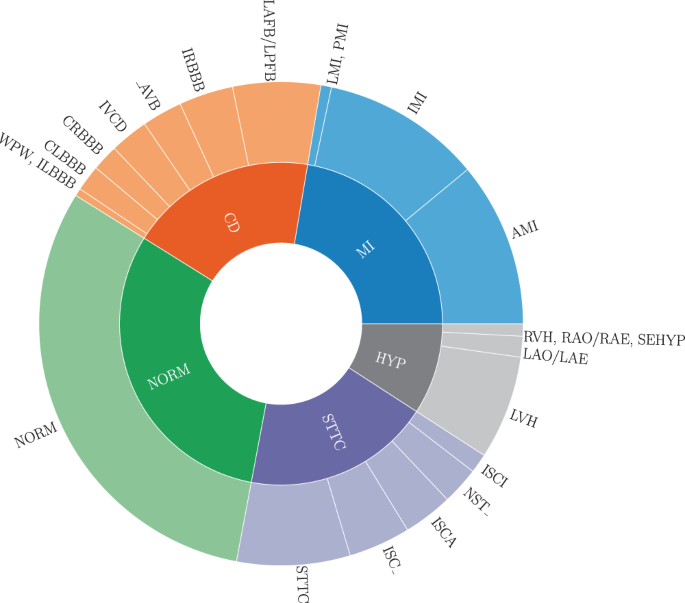
\includegraphics[width=0.5\textwidth]{Definitions/ptb-xl.jpeg}
\caption{Class Distribution for PTB-XL data set}
\label{fig:CD-ptbxl}
\end{figure} 


\section{Results}

Several methods exist in the literature to evaluate a DL classifier. We evaluate our classifiers using accuracy, area under curve (AUC), confusion matrix, sensitivity, and specificity. A detail of the results obtained by applying each of the algorithms and the respective data set is explained in this section. 
%%%%%%
In the sequel, we present the results acquired for each data set and also compare our results to the other state-of-the-art work. An overview of the section is presented in Table \ref{tbl:overview}.

\subsection{ECG HAR data set}
The data set was trained initially using a plain LSTM to compare the model performance with the previous experiments. The data was fed into the model without any pre-processing. The LSTM initially gave an accuracy of 49.80\% which was increased to 54\% by fine tuning the hyperparameters. In the previous experiments, extensive pre-processing was carried out to extract the related features and then those features were fed into the model. That approach though gave excellent accuracy but was not automated. LSTMs have been shown to have a sense of previous timestamps or history in the time series, but CNNs have superior feature extraction capability. To test our hypothesis, a CNN was placed on top of the LSTM layer. The accuracy immediately improved to 93\%. After some fine tuning the hyperparameters and adjusting the number of CNN layers, the validation accuracy got better than the state-of-the-art results. A testing accuracy of 99.21\%-100\% was achieved and a validation accuracy of 99.21\% was achieved.
For the first data set, the results were almost perfect with a validation accuracy of 99.21\% and a testing accuracy of 99.21\%-100\%. The previous work achieved similar accuracy but with transfer learning and pre-processing the signals by converting them into wavelet transforms and then into scalograms. This model achieves similar accuracy even by avoiding all those steps.
The following Table~\ref{tbl:conf} shows the confusion matrix for the testing data set showing an almost perfect accuracy of 99.22\%.

\begin{table}[!ht]
	\caption{Confusion Matrix for Fall Detection ECG data set using CNN-LSTM (Algorithm~\ref{alg:algorithm1})}
	\label{tbl:conf}
	\tiny
	\centering
	\scriptsize
	\renewcommand{\arraystretch}{1.2}
	\begin{tabular}{cr|ccc}
		\multicolumn{2}{c}{}
		&   \multicolumn{3}{c}{Actual} \\
		&        
		&\rotatebox{90}{ DA} 
		&\rotatebox{90}{ Fall} 
		&\rotatebox{90}{ Rest} 
	
	 \\	
		\cline{2-5}
		\multirow{3}{*}{\rotatebox[origin=c]{90}{Predicted}}
		%&DA    & 30    &0     &0  	\\ 
		%&Fall  & 0     &53     &0  	 \\ 
		%&Rest  & 0     &0  	& 45	  \\ 
	    &DA    & 30    &0     &0  	\\ 
		&Fall  & 1     &52     &0  	 \\ 
		&Rest  & 0     &0  	& 45	  \\ 
		
		%\cline{2-6}
	\end{tabular}
% % Original data from :http://10.18.2.21:8888/notebooks/Implementation1_CNN_LSTM_original.ipynb
\end{table}

Fall detection using ECG signals was also done by applying Algorithm~\ref{alg:algorithm2} to the HAR data set. Each sequence in the data set consists of 4000 time stamps. The initial tensor size was [1273, 1, 4000], which is of the format [Total Sequences, Number of features, Sequence length]. Each of the ECG sequences was divided into 100 chunks of 40 time stamps each, and then wavelet transform was calculated for each chunk resulting in a final dimension of [1273, 108, 40]. The model was trained in 403.39 seconds. The result is again achieved without any manual feature extraction or transfer learning model. 
The following Table~\ref{tbl:confatt} shows the confusion matrix for the testing data set showing also accuracy of 95.31\% %97.66\%.
%\begin{figure}[H]
%\centerline{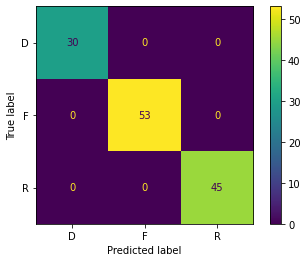
\includegraphics[width=18.5pc]{Definitions/cm-100.png}}
%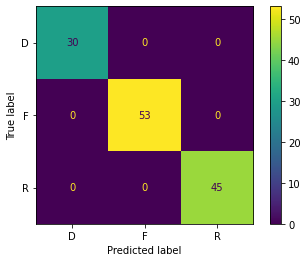
\includegraphics[width=10.5 cm]{Definitions/cm-100.png}
%\caption{Confusion Matrix for Fall Detection ECG data set showing a Testing Accuracy of 100\% \label{fig4}}
%\end{figure}   
%%%%
\begin{table}[!ht]
    % Original data from http://10.18.2.21:8888/notebooks/Attention_HAR.ipynb
	\caption{Confusion Matrix for Fall Detection ECG data set using Attention (Algorithm~\ref{alg:algorithm2})}
	\label{tbl:confatt}
	\tiny
	\centering
	\scriptsize
	\renewcommand{\arraystretch}{1.2}
	\begin{tabular}{cr|ccc}
		\multicolumn{2}{c}{}
		&   \multicolumn{3}{c}{Actual} \\
		&        
		&\rotatebox{90}{ DA} 
		&\rotatebox{90}{ Fall} 
		&\rotatebox{90}{ Rest} 
	
	 \\	
		\cline{2-5}
		\multirow{3}{*}{\rotatebox[origin=c]{90}{Predicted}}
		&DA    &29  &1   &0 \\ 
		&Fall  &2   &49 &2  \\ 
		&Rest  &0   &0  &44 \\ 
		%\cline{2-6}
	\end{tabular}
\end{table}
\subsection{PTB Diagnostics} 

Algorithm~\ref{alg:algorithm1}, i.e.\ CNN-LSTM was used to model PTB diagnostic to differentiate normal from abnormal heartbeats. Previous studies have emphasised feature extraction before feeding into the neural network, or transfer learning where the model is initially trained with an existing data set and later on trained with the same learned weights on the desired data set such as in \cite{9630333}. In the current benchmark for MI classification using PTB diagnostic, ConvNetQuake neural network model was adapted to achieve an accuracy of 99.44\%. Similarly, heavy pre-processing like wavelet transformation \cite{ACHARYA2017190}, data balancing \cite{latest},  or transfer learning \cite{8419425} is used in the literature to achieve higher accuracy for ECG signal classification. In our work, no pre-processing to the individual readings were applied and the model achieving 99.66\% accuracy, exceeds the state-of-the-art accuracy for normal versus abnormal classification which was previously 99.43\%. 

Algorithm~\ref{alg:algorithm2}, i.e.\ the attention /transformer model was also used to model PTB diagnostic to differentiate normal from abnormal heart beats. This yields an accuracy of 99.73\%, a precision of 99.73\%, a sensitivity of 99.2\%, and a specificity of 99.91\%.

The confusion matrices of both algorithms are depicted in Table~\ref{tbl:ConfusionMatrixPTB} below. %and \ref{tbl:ConfusionMatrixPTBPercentage}

\begin{table}[!ht]
	\caption{Confusion Matrices for PTB data set}
	\label{tbl:ConfusionMatrixPTB}
\centering
\scriptsize
{%
	\renewcommand{\arraystretch}{1.5}
	\begin{tabular}{cr|r r | r r}
		\multicolumn{2}{c}{}
		&   \multicolumn{4}{c}{Predicted}\\
		\multicolumn{2}{c|}{}
		&   \multicolumn{2}{c|}{Algorithm~\ref{alg:algorithm1}} &   \multicolumn{2}{c}{Algorithm~\ref{alg:algorithm2}}\\
		\cline{3-6}
		&	&\multicolumn{1}{c}{\rotatebox{90}{NORMAL}} &\multicolumn{1}{c|}{\rotatebox{90}{ABNORMAL }}&\multicolumn{1}{c}{\rotatebox{90}{NORMAL}} &\multicolumn{1}{c}{\rotatebox{90}{ABNORMAL }}\\
		\cline{2-6}
		\multirow{2}{*}{\rotatebox[origin=c]{90}{Actual}}
		& NORMAL 	&371	&1		&372	&1	\\	
		& ABNORMAL 	&2	    &1081	&3		&1080\\ 
	\end{tabular}
}
%data from http://10.18.2.21:8888/notebooks/ptb_cnn_lstm.ipynb
\end{table}

%%%CM with percentages
%\begin{table}[!ht]
%	\caption{Confusion Matrix for PTB data set using CNN-LSTM (Algorithm~\ref{alg:algorithm1}) Percentage}
%	\label{tbl:ConfusionMatrixPTBCNNLSTMPercentage}
%\centering
%\scriptsize

%{%
%	\renewcommand{\arraystretch}{1.5}
%	\begin{tabular}{cr|r r}
%		\multicolumn{2}{c|}{}
%		&   \multicolumn{2}{c}{Predicted}\\
%		&	&\multicolumn{1}{c}{\rotatebox{90}{NORMAL}} &\multicolumn{1}{c}{\rotatebox{90}{ ABNORMAL}}\\
%		\cline{2-4}
%		\multirow{2}{*}{\rotatebox[origin=c]{90}{Actual}}
%		& NORMAL 	&99.73	&0.27	\\	
%		& ABNORMAL 	&0.28	&99.72\\ 
%	\end{tabular}
%}
%\end{table}
%%%%%%%

In comparison to CNN-LSTM, i.e.\ Algorithm~\ref{alg:algorithm1}, the attention model with wavelet embedding has shown to be more efficient as it uses fewer parameters and less training time as compared to CNN-LSTM model as shown in Table~\ref{tbl:attvscnnlstm}. However, the time and number of parameters for Algorithm~\ref{alg:algorithm2} might increase eventually with the increase in the number of attention heads and encoder layers.

\begin{table}[!ht]
\centering
\caption{Comparison between Attention model with wavelet embedding and CNN-LSTM hyper parameters and performance
\label{tbl:attvscnnlstm}}
\begin{tabular}{ll|l|l|l|l|}
\cline{3-6}
\multicolumn{2}{l|}{}                                                   & {\rotatebox{90}{Total Parameters}} & {\rotatebox{90}{Training Time}} & {\rotatebox{90} {Learning Rate}} & {\rotatebox{90} {Epochs}} \\ \hline
\multicolumn{1}{|l|}{\multirow{2}{*}{HAR}}            & Attention Model &  \textbf{ 461,583}               &   \textbf{403.39 s}            &     0.00002         & 500        \\ \cline{2-6} 
\multicolumn{1}{|l|}{}                                & CNN-LSTM        &      2,471,503            &       80.56 s          &     0.001       & 100        \\ \hline
\multicolumn{1}{|l|}{\multirow{2}{*}{PTB}} & Attention Model &  \textbf{61762}              &   \textbf{823.54s}            &       0.001        &     1000   \\ \cline{2-6} 
\multicolumn{1}{|l|}{}                                & CNN-LSTM        &         210,025         &   1923.87 s            &   0.001            & 1000       \\ \hline
\end{tabular}
\end{table}

Multiple metrics were used to evaluate the performance of the model. The terms $tp$, $fp$, $tn$, and $fn$ refer to true positive, false positive, true negative, and false negative respectively. Since in medical terminology, true positive would refer to the medical condition being diagnosed, $tp$ in our context refers to the diagnosis of MI. The performance metrics were calculated using following formulas:
\begin{align*} 
%paper to be referred: A systematic analysis of performance measures for classification tasks
Accuracy    &=(tp + tn)/(tp + fp + fn + tn)   \\
Precision   &=tp/(tp + fp)                   \\
Sensitivity &=tp/(tp + fn)               \\
Specificity &=tn/(tn + fp)    
\end{align*}

 
The results for our leading models are summarized in Table~\ref{tbl:kpis}.
\begin{table}[!ht]
\caption{Metrics for leading CNN-LSTM and Attention}
\label{tbl:kpis}
\centering
\scriptsize
{%
	\renewcommand{\arraystretch}{1.5}
	\begin{tabular}{cr|r r}
		\multicolumn{2}{c|}{}
		&   \multicolumn{2}{c}{Predicted}\\
		&	&\multicolumn{1}{c}{\rotatebox{90}{CNN-LSTM}} &\multicolumn{1}{c}{\rotatebox{90}{ ATTENTION}}\\
		\cline{2-4}
		\multirow{2}{*}{\rotatebox[origin=c]{90}{Actual}}
		& Accuracy 	    &99.79	    &	99.73\\	
		& Precision 	&99.91	    &	99.91\\	
		& Sensitivity 	&99.81	    &	99.72\\	
		& Specificity 	&99.73	    &	99.73\\	
	\end{tabular}
\medskip	
}
\end{table}

Fig.~\ref{fig:trainigValidationGraph} and Fig.~\ref{fig:trainingAndValidationLossAttentionModel} show examples of training accuracy and losses for PTB dataset, respectively.
\begin{figure}[!ht]	
\caption{Training and validation graph over epochs for the PTB data set for Algorithm~\ref{alg:algorithm1}}
\label{fig:trainigValidationGraph}
\centerline{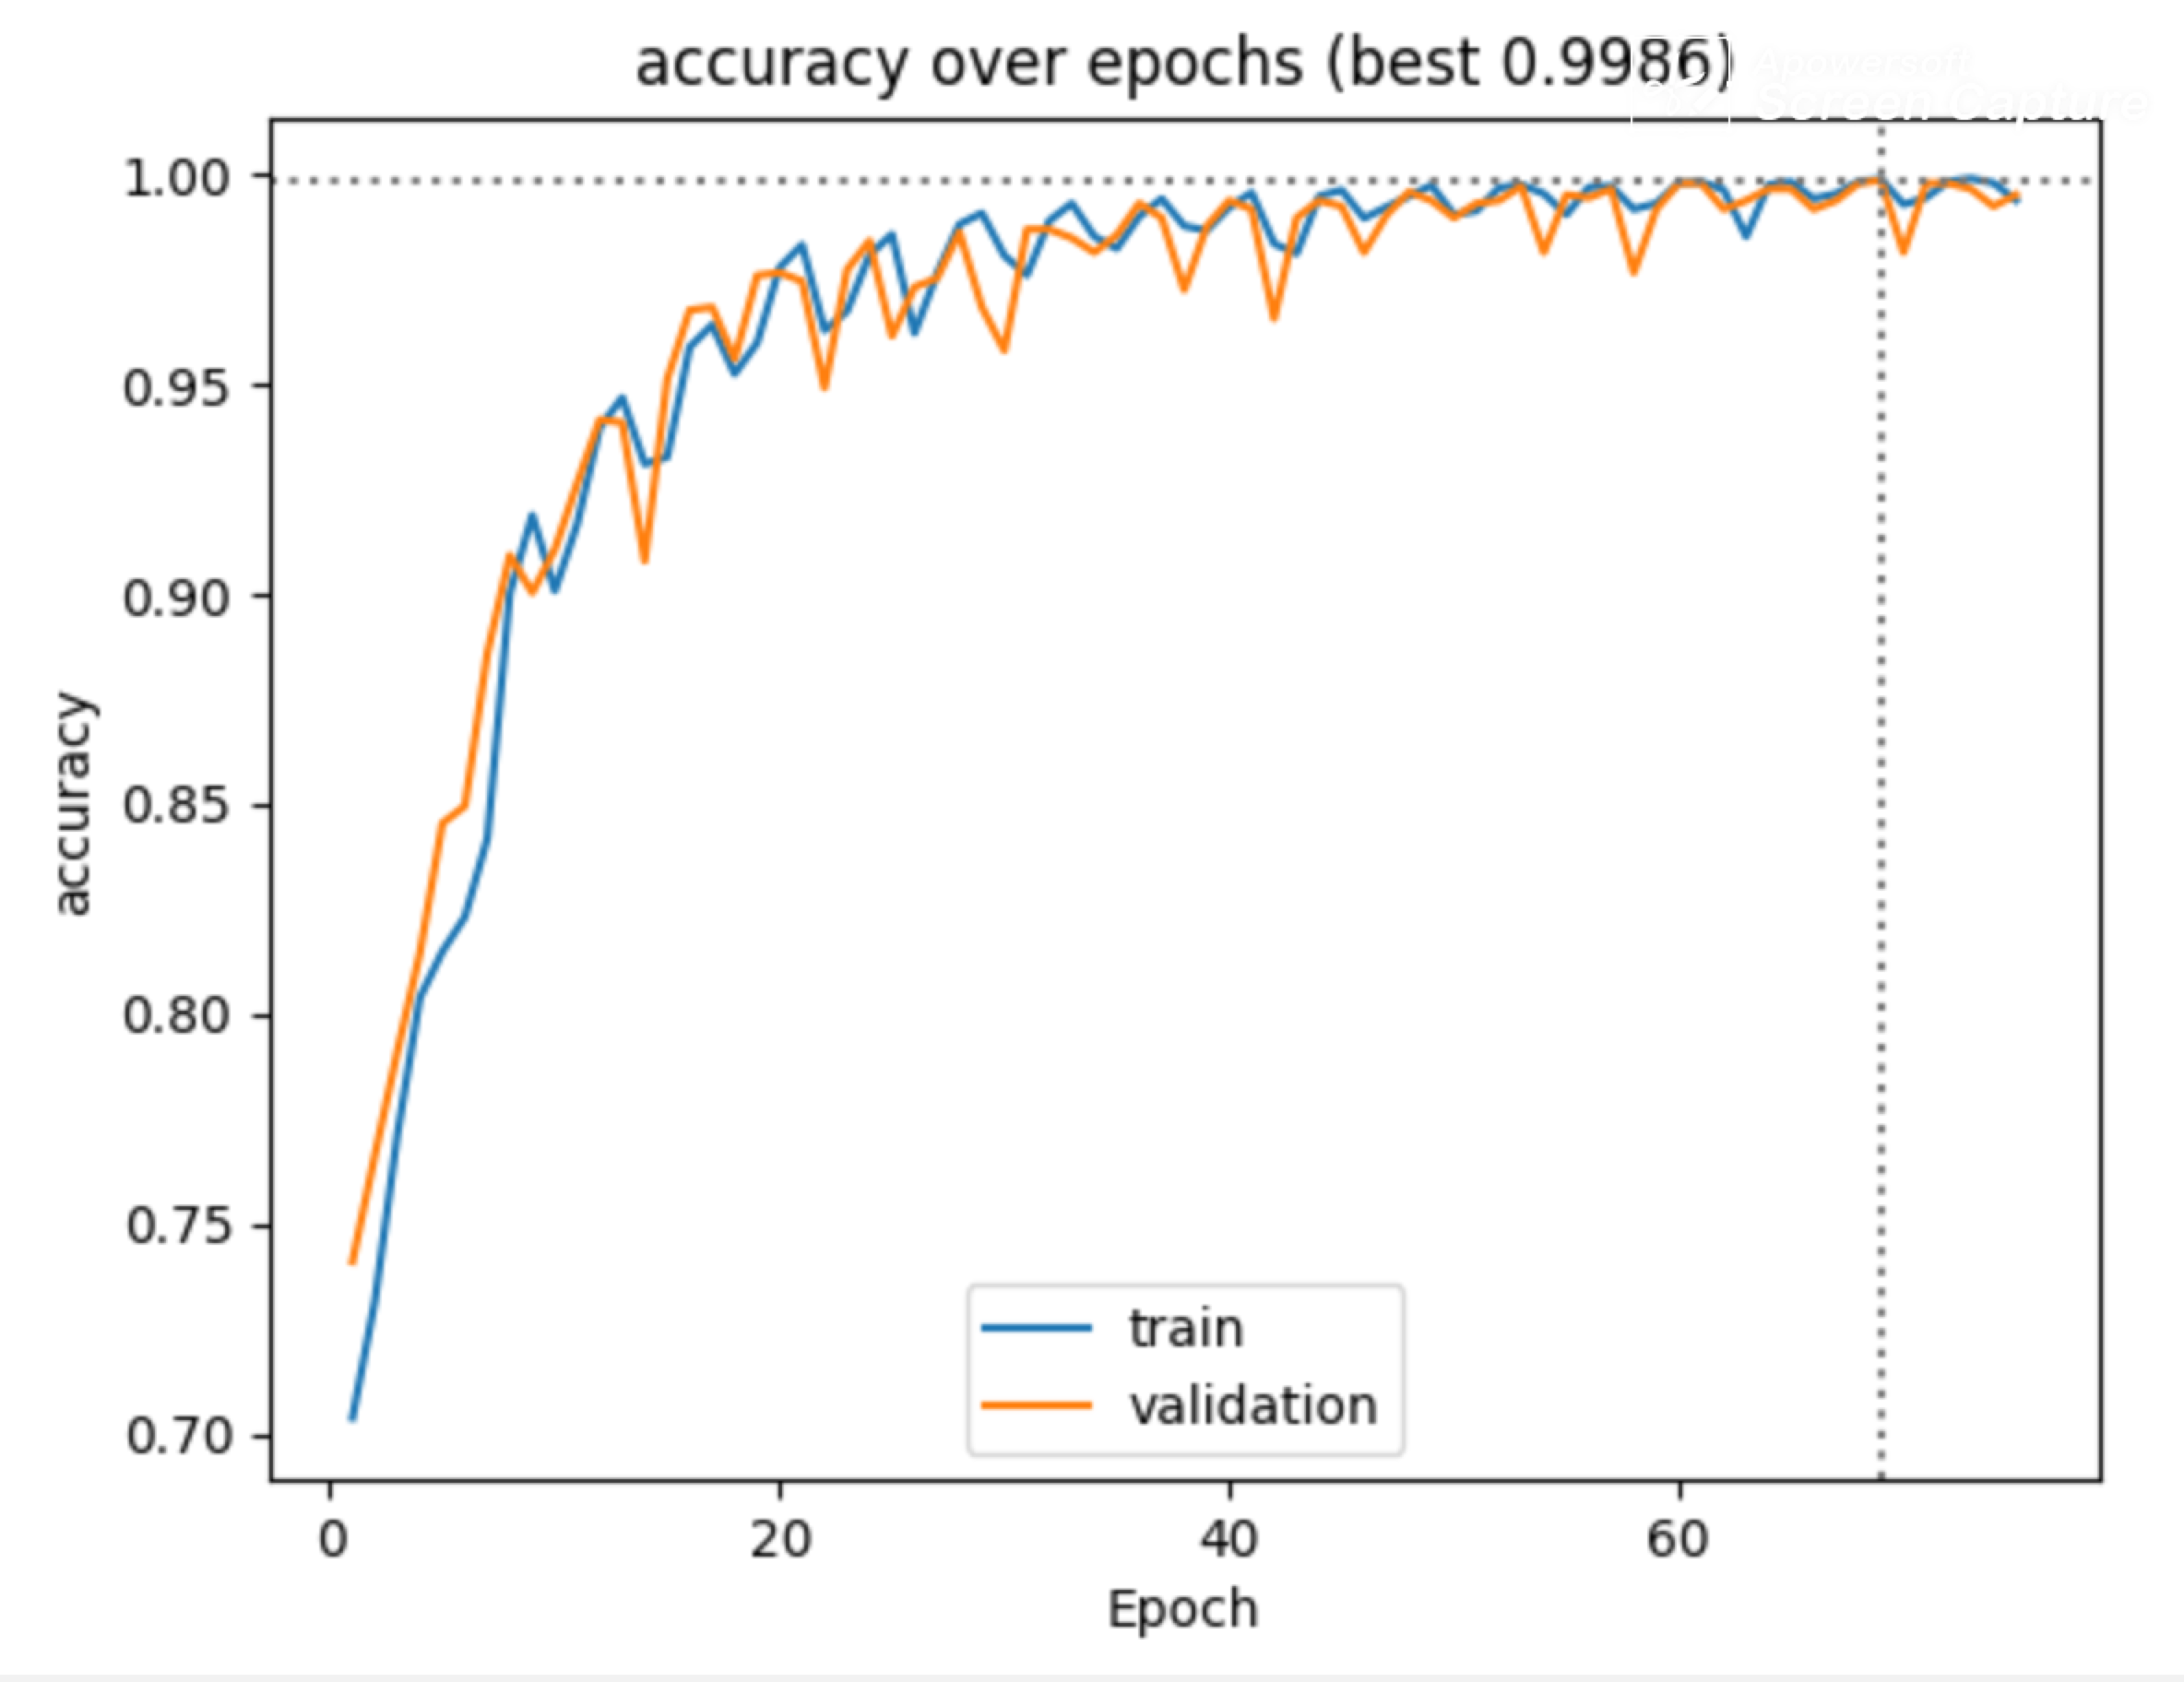
\includegraphics[width=18.5pc]{Definitions/PTB_training.png}}
%\widefigure
%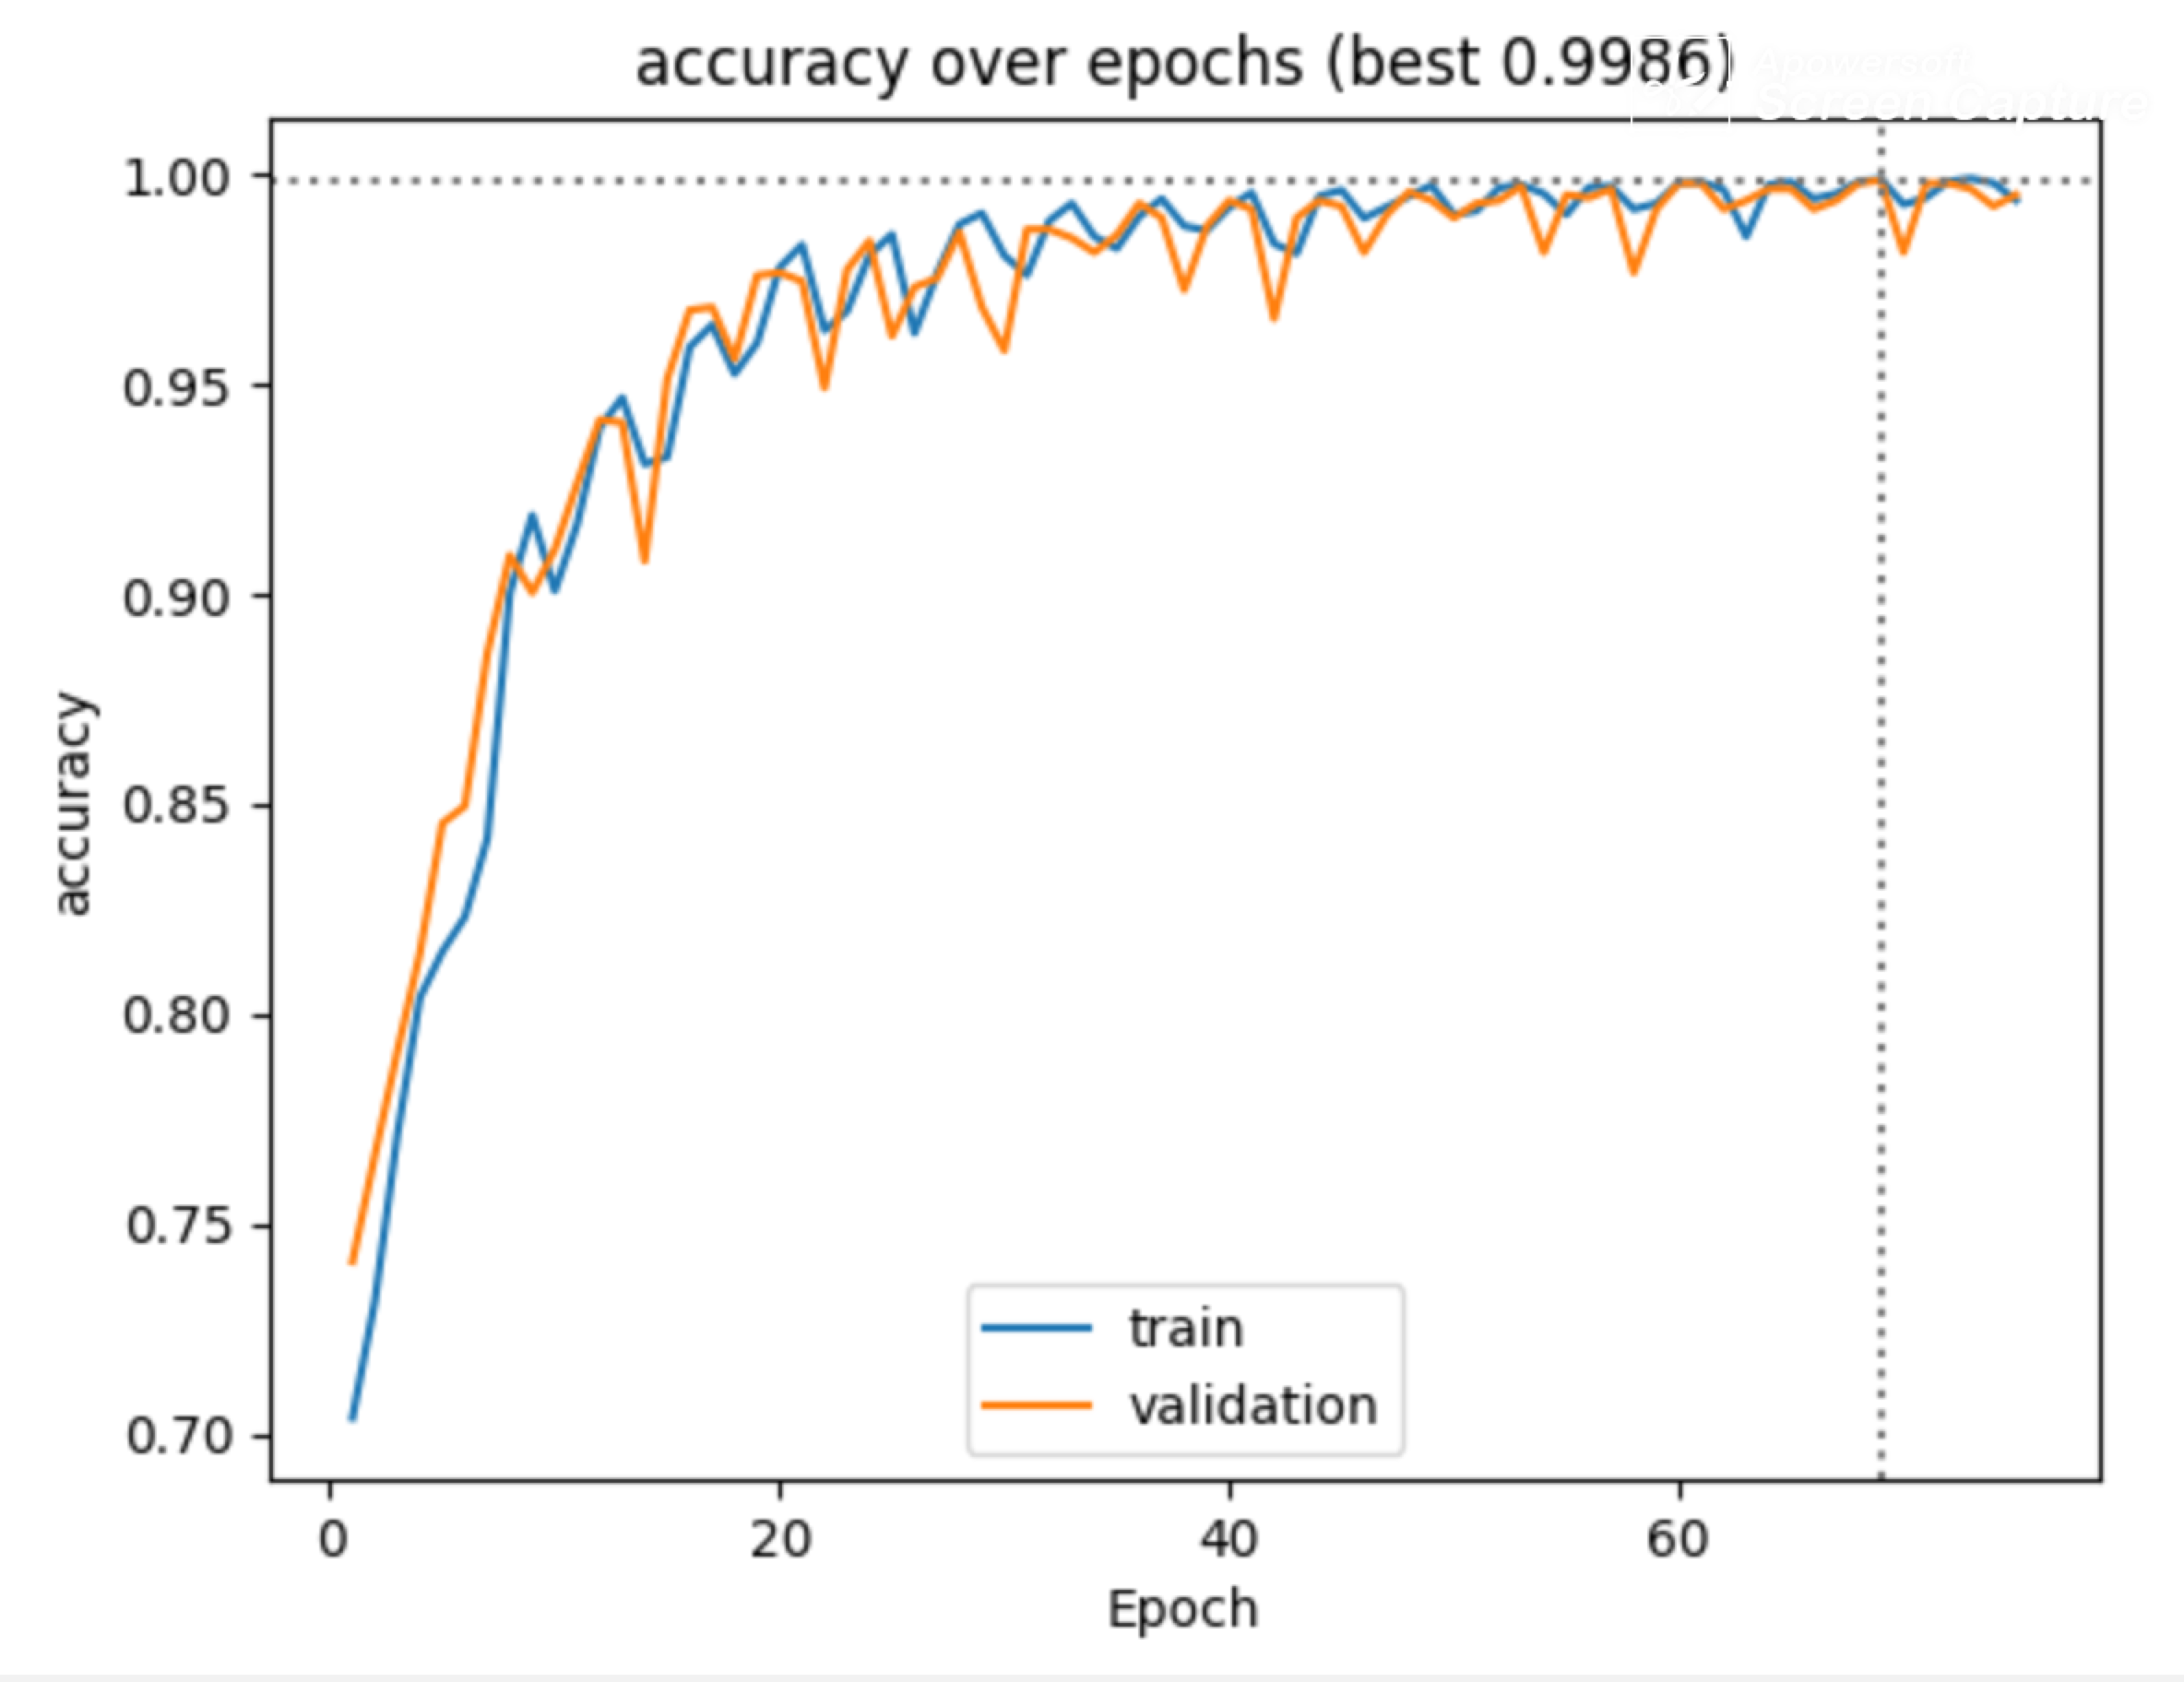
\includegraphics[width=15 cm]{Definitions/PTB_training.png}
\end{figure}


\begin{figure}[!ht] % from http://10.18.2.21:8888/notebooks/attenstion-ptb11.ipynb
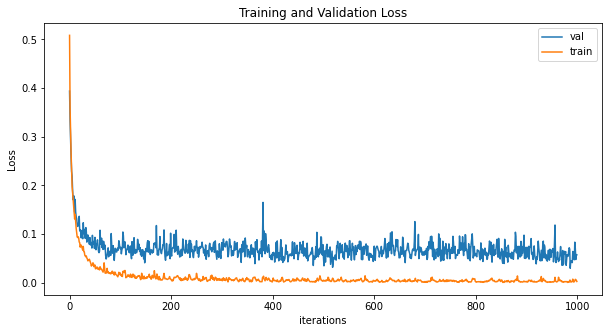
\includegraphics[width=0.45\textwidth]{Images/TrainingValidationLossAttention}
\caption{Training and Validation Loss for the PTB data set for Algorithm~\ref{alg:algorithm2}}
\label{fig:trainingAndValidationLossAttentionModel}
\end{figure}    

\subsection{PTB XL Diagnostics}
Since PTB XL is a relatively new data set, many recent studies using this data set adapt it for different classification tasks such as super diagnostic, sub diagnostic, form, etc. For our study, 5 super diagnostic (SD) classes were classified. A validation accuracy of 75.70\% and a testing accuracy of 74.33\% were achieved. AUC score of 0.8395 was achieved, see Table~\ref{tbl:perfIndicators}. 

%\lipsum[2-5]
\begin{table}[ht]
\caption{Performance indicators}
\label{tbl:perfIndicators}
\centering
 \begin{tabular}{|c c c c|} 
 \hline
 Classification classes & \rotatebox{90}{Val. Accuracy} & \rotatebox{90}{Testing Accuracy} &\rotatebox{90}{AUC score} \\ [0.5ex] 
 \hline\hline
 Super-diagnostic Classes  & 75.70\% & 74.33\% & 0.8395 \\ 
 %Sub diagnositic Classes  & -- & -- & -- \\
 MI vs. Normal Class & 90.94\% & 89.1\% & 0.87 \\
 MI vs. Super-diagnostic classes & 91.07\% & 90.2\% & 0.762 \\
  [1ex] 
 \hline
 \end{tabular}
\end{table}

\bigskip
 A direct comparison to the state-of-the-art is not very straightforward for PTB-XL mainly because it is a newer data set and many new studies, which use it, focus on different classification tasks. Though our results for this data set do not beat the state-of-the-art accuracy, the results are still comparable. Virginia et al.~\cite{S2021102779} and Martin et.al~\cite{MARTIN2021102179} achieved an accuracy of 90.8\% and 77.12\%  for MI classification respectively. Similarly, Śmigielet al.~\cite{s21248174} achieved an accuracy of 78.0–75.2\% for 5 class classification. 
 
 Our Algorithm~\ref{alg:algorithm1} applied for myocardial infarction detection using PTB XL data set yields a validation accuracy of 90.94\% when it is MI versus normal class in super diagnostic, and 91.27\% when it is MI vs other 4 superclasses. Please note the AUC as a metric was calculated only for PTB-XL data set as it is used widely for comparison of this particular data set in the literature. 
The experiment with Algorithm~\ref{alg:algorithm2} on multi-lead data sets such as PTB XL is still in a preliminary stage and requires further investigation on how to merge the natural domain dimension of multi-lead with the dimensional embedding technique. However, similar results for another research project of ours yield promising results for the Algorithm~\ref{alg:algorithm2} with a multidimensional or multi-featured data set, see \cite{Schaefer}. Henceforth these experiments have not been mentioned and as work in progress will be published in a future contribution.
\subsection{Summary}
As seen in Table~\ref{tbl:tbl3}, our model leads in almost all of the evaluation criteria for the classification of PTB data set.

%\section{Theoretical Explanation for the CNN-LSTM prediction- A proposal }
\begin{table*}[t]
    \centering%
    \caption{Our result compared with other similar studies in literature which used PTB database(Built upon \cite{10.1007/978-3-030-64610-3_40})}
    \label{tbl:tbl3}
    \small
    \begin{tabular}{*{5}{p{.16\textwidth}}}
          \toprule
    \textbf{Work} &\textbf{Accuracy(\%)} &  \textbf{Sensitivity(\%)} &\textbf{Specificity(\%)} &\textbf{Precision(\%)}
      \\\midrule
    Acharya et al. \cite{ACHARYA2017190} & 93.5 & 93.7 & - & 92.8\\
      %\\\midrule
     Safdarian et al. \cite{safdarain} &94.7 & - & - & -\\
       %\\\midrule
     Kojuri et al. \cite{kojuri}&95.6 & 93.3 & - & 97.9 \\
     %\\ \midrule 
     Sun et al. \cite{sun} & - & 92.6 & - & 82.4\\
      Liu et al. \cite{Liu94}& 94.4 & - & - & -\\
      Sharma et al. \cite{Sharma2018InferiorMI}& 96 & 93 & - & 99\\
      Kachuee et al. \cite{8419425}& 95.9 & 95.1 & - & 95.2\\
      Remya et al. \cite{remya}& 93.61 & 93.22 & 94.28 & -\\
    Reasat et al. \cite{reasat}& 84.54 & 85.33 & 84.09 & -\\
     Zewdie et al. \cite{zewdie2014fully}& 98.3 & 98.7 & 96.4 & -\\
      Feng et al. \cite{feng}& 95.4 & 98.2 & 86.5 & -\\
      Strodthoff et al. & - & 93.3 & 89.7 & -\\
      Huang et al.& 96.96 & 99.89 & 92.51 & 95.35\\
      Liu et al. \cite{liu} & 98.59 & 99.53 & 94.50 & -\\
     Gupta et al.\cite{10.1007/978-3-030-64610-3_40} & 99.43 & 99.40 & 99.45 & 99.46\\
     Ours (CNN-LSTM)& \textbf{99.93} & \textbf{99.81} & 99.73 & \textbf{99.91}\\
     Ours (Attention) & \textbf{99.73} & 99.72 & \textbf{99.73} & \textbf{99.91}\\    
     %\\ \midrule
     \bottomrule
    \end{tabular}
\end{table*}

\begin{table*}[!ht]
    \centering%
    \caption{Overview of the experiments with different data sets and the
acquired performances}
    \label{tbl:overview}
    \small
    \begin{tabular}{*{5}{p{.16\textwidth}}}
          \toprule
    \textbf{Classification task} &\textbf{Data set} &  \textbf{Achieved Accuracy} &\textbf{Algorithm} &\textbf{State-of-the-art accuracy}
      \\\midrule
     Fall detection & ECG HAR  & 99.21\% & Attention & 98.44\% \cite{2021}\\
      %\\\midrule
     Fall detection & ECG HAR  & 99.21\% & CNN-LSTM & 98.44\%\cite{2021}\\
     MI detection & PTB  & 99.73\% & Attention & 99.44\%\cite{10.1007/978-3-030-64610-3_40}  \\
     MI detection & PTB  & 99.93\% & CNN-LSTM & 99.44\%\cite{10.1007/978-3-030-64610-3_40} \\
       %\\\midrule
    SD Class & PTB XL & 75.70\% & CNN-LSTM & - \\
     %\\ \midrule 
     MI detection & PTB XL & 91.07\% & CNN-LSTM & -\\
      
      
     %\\ \midrule
     \bottomrule
    \end{tabular}
\end{table*}
%DONE\todo{compare and cosolidate metrics from table 9 and table 7}
\section{Discussion}
As mentioned earlier, state-of-the-art accuracy's are achieved using CNN-LSTM model for three data sets and the attention model for PTB data set. In similar previous works, mostly one set of experiments is performed with a single database to prove the usability of the models. However, we worked on three data sets separately. The first data set is used for the classification of human activities including falls. The second one consists of extracted heartbeats for the classification of MI vs normal heartbeats. The third one consists of a 12-lead ECG data set for multiple cardiovascular conditions. The success of our proposed algorithms on all three data sets generalizes its usefulness for ECG classifications over multiple tasks.

Hybrid models help to combine the features of the base models. This is often more powerful than very deep models with hundreds of layers because for medium-sized data sets, deeper models tend to over-fit. A LSTM model keeps track of the past trends in the time series and can also help in the prediction of the next time stamps. In our study, the results of the CNN-LSTM model have shown to be always better than both of the models implemented individually. This was verified for the HAR data set by \cite{Pusch} and we compare the results from Table~\ref{tbl:tbl3} for PTB data set where multiple variations of CNN and LSTMs have been applied separately in the previous works.
The performance of the model on HAR data set is observed to increase up to a certain level with the increase in a) the number of filters in conv1d layer for CNN-LSTM and b) the number of dimensions in the dimensional embedding with the attention model. Since the data set is not very large, a final conclusion cannot be drawn at this stage but it merits further investigation. 
The attention algorithm clearly has a computational advantage over CNN-LSTM algorithm as seen in Table~\ref{tbl:attvscnnlstm}. It takes less time to converge and even has fewer parameters to train than the CNN-LSTM algorithm.
Our work presents the following advantages:
\begin{itemize}
  \item A hybrid CNN-LSTM model and attention with discrete wavelet transformation as an embedding are proposed.
  \item No or very little manual feature extraction is required for training the model.
  \item Three publicly available data sets are used separately for the training using the proposed models.
  \item State-of-the-art accuracy of 99.86\% and 99\% is achieved for the PTB dataset and ECG for HAR classification respectively without any feature extraction or pre-processing.

\end{itemize}
Hence, we did address our research question and achieved results equivalent to many recent studies without any pre-processing or feature extraction. We have also shown to train the models in an efficient manner computationally.



%%%%%%%%%%%%%%%%%%%%%%%%%%%%%%%%%%%%%%%%%%
\vspace{6pt} 



\section{CONCLUSION}

The models proposed and explained in this paper aim to better classify ECG time series for different conditions using minimum pre-processing steps. The availability of publicly available data sets have made it possible to verify the robustness and usefulness of the proposed models via achieving state-of-the-art accuracy using multiple data sets. This would eventually help medical practitioners to identify multiple heart conditions in an automatic manner with minimum feature extraction. Specifically for the MI classification, since the results are close to 100\% the model is ready to be deployed for medical evaluation. 

\section{Data and Code Availability}
The data sets used are publicly available and present in the corresponding repositories:
\begin{itemize}
\item ECG HAR dataset : \cite{ info12020063-20}
\item PTB DB dataset : \cite{ptb}
\item PTB XL : \cite{ptbxl}
\end{itemize}

The code is available on GitHub at \url{https://github.com/buttfatimasajid/Towards-Automated-Feature-Extraction-For-Deep-Learning-Classification-of-Electrocardiogram-Signals}.

\section{ACKNOWLEDGMENT}

The authors thank Kylie Pusch who contributed some ideas in her bachelor thesis \cite{Pusch}. This work was supported in part by the PhD-research program of the Faculty of Computer Science and Engineering Fb2 of Frankfurt University of Applied Sciences.
%=====================================
% References, variant A: external bibliography
%=====================================




\begin{thebibliography}{1}
\bibitem{cite-key}Wagner, P., Strodthoff, N., Bousseljot, R., Kreiseler, D., Lunze, F., Samek, W. \& Schaeffter, T. PTB-XL, a large publicly available electrocardiography dataset. {\em Scientific Data}. \textbf{7}, 154 (2020), \url{https://doi.org/10.1038/s41597-020-0495-6}


\bibitem{cdc}Centers for Disease Control and \& Prevention ,Underlying Cause of Death, 1999-2020 Request,  \url{https://wonder.cdc.gov/ucd-icd10.html}
\bibitem{fallcardio}Tan, M. \& Kenny, R. Cardiovascular Assessment of Falls in Older People. {\em Clinical Interventions In Aging}. \textbf{1} pp. 57-66 (2006,2)

\bibitem{9630333}Yang, F., Wang, G., Luo, C. \& Ding, Z. Improving Automatic Detection of ECG Abnormality with Less Manual Annotations using Siamese Network. {\em 2021 43rd Annual International Conference Of The IEEE Engineering In Medicine Biology Society (EMBC)}. pp. 1120-1123 (2021)
\bibitem{9190034}Strodthoff, N., Wagner, P., Schaeffter, T. \& Samek, W. Deep Learning for ECG Analysis: Benchmarks and Insights from PTB-XL. {\em IEEE Journal Of Biomedical And Health Informatics}. \textbf{25}, 1519-1528 (2021)
\bibitem{7164783} Jambukia, S., Dabhi, V. \& Prajapati, H. Classification of ECG signals using machine learning techniques: A survey. {\em 2015 International Conference On Advances In Computer Engineering And Applications}. pp. 714-721 (2015)

\bibitem{karpagachelvi2010ecg}Karpagachelvi, S., Arthanari, M. \& Sivakumar, M. ECG Feature Extraction Techniques - A Survey Approach. (arXiv,2010), \url{https://arxiv.org/abs/1005.0957}
\bibitem{2021}Butt, F., La Blunda, L., Wagner, M., Schäfer, J., Medina-Bulo, I. \& Gómez-Ullate, D. Fall Detection from Electrocardiogram (ECG) Signals and Classification by Deep Transfer Learning. {\em Information}. \textbf{12}, 63 (2021,2), \url{http://dx.doi.org/10.3390/info12020063}
\bibitem{ECGdb}Kim, Y., Shin, D., Park, M., Lee, S., Jeon, M., Yoon, D. \& Park, R. ECG-ViEW II, a freely accessible electrocardiogram database. {\em PloS One}. \textbf{12}, e0176222 (2017), \url{https://europepmc.org/articles/PMC5402933}
\bibitem{ysnc-gc65-20}Kher, R. Wearable Ambulatory Electrocardiogram (ECG) and EEG dataset. (IEEE Dataport,2020), \url{https://dx.doi.org/10.21227/ysnc-gc65}
\bibitem{article}Dallali, A., Kachouri, A. \& Samet, M. A Classification of Cardiac Arrhythmia Using WT, HRV, and Fuzzy C-Means Clustering. {\em Signal Processing: An International Journal (SPJI)}. \textbf{Volume (5)} pp. 101-108 (2011,1)
\bibitem{10.1007/978-3-030-64610-3_40}Gupta, A., Huerta, E., Zhao, Z. \& Moussa, I. Deep Learning for Cardiologist-Level Myocardial Infarction Detection in Electrocardiograms. {\em 8th European Medical And Biological Engineering Conference}. pp. 341-355 (2021)
\bibitem{article2}Khorrami, H. \& Moavenian, M. A comparative study of DWT, CWT and DCT transformations in ECG arrhythmias classification. {\em Expert Syst. Appl.}. \textbf{37} pp. 5751-5757 (2010,8)

%NOT refered
%\bibitem{article3}Korürek, M. \& Doğan, B. ECG beat classification using particle swarm optimization and radial basis function neural network. {\em Expert Systems With Applications}. \textbf{37} pp. 7563-7569 (2010,12)
\bibitem{7019490}Sathyapriya, L., Murali, L. \& Manigandan, T. Analysis and detection R-peak detection using Modified Pan-Tompkins algorithm. {\em 2014 IEEE International Conference On Advanced Communications, Control And Computing Technologies}. pp. 483-487 (2014)
\bibitem{cite-key1}Khan, A., Sohail, A., Zahoora, U. \& Qureshi, A. A survey of the recent architectures of deep convolutional neural networks. {\em Artificial Intelligence Review}. \textbf{53}, 5455-5516 (2020), \url{https://doi.org/10.1007/s10462-020-09825-6}
\bibitem{8308186}Albawi, S., Mohammed, T. \& Al-Zawi, S. Understanding of a convolutional neural network. {\em 2017 International Conference On Engineering And Technology (ICET)}. pp. 1-6 (2017)
\bibitem{9233318}Blunda, L., Gutiérrez-Madroñal, L., Wagner, M. \& Medina-Bulo, I. A Wearable Fall Detection System Based on Body Area Networks. {\em IEEE Access}. \textbf{8} pp. 193060-193074 (2020)
\bibitem{EBRAHIMI2020100033}Ebrahimi, Z., Loni, M., Daneshtalab, M. \& Gharehbaghi, A. A review on deep learning methods for ECG arrhythmia classification. {\em Expert Systems With Applications: X}. \textbf{7} pp. 100033 (2020), \url{https://www.sciencedirect.com/science/article/pii/S2590188520300123}
\bibitem{cui2016multiscale}Cui, Z., Chen, W. \& Chen, Y. Multi-Scale Convolutional Neural Networks for Time Series Classification.  {\em ArXiv}. \textbf{abs/1603.06995}(2016)
\bibitem{8419425}Kachuee, M., Fazeli, S. \& Sarrafzadeh, M. ECG Heartbeat Classification: A Deep Transferable Representation. {\em 2018 IEEE International Conference On Healthcare Informatics (ICHI)}. pp. 443-444 (2018)
\bibitem{e23010119}Wang, T., Lu, C., Sun, Y., Yang, M., Liu, C. \& Ou, C. Automatic ECG Classification Using Continuous Wavelet Transform and Convolutional Neural Network. {\em Entropy}. \textbf{23} (2021), \url{https://www.mdpi.com/1099-4300/23/1/119}
\bibitem{ACHARYA2017190}Acharya, U., Fujita, H., Oh, S., Hagiwara, Y., Tan, J. \& Adam, M. Application of deep convolutional neural network for automated detection of myocardial infarction using ECG signals. {\em Information Sciences}. \textbf{415-416} pp. 190-198 (2017), \url{https://www.sciencedirect.com/science/article/pii/S0020025517308009}
\bibitem{2019}Strodthoff, N. \& Strodthoff, C. Detecting and interpreting myocardial infarction using fully convolutional neural networks. {\em Physiological Measurement}. \textbf{40}, 015001 (2019,1), \url{http://dx.doi.org/10.1088/1361-6579/aaf34d}


\bibitem{zheng}Zheng Y., Liu Q., Chen E., Ge Y., Zhao J.L. (2014) Time Series Classification Using Multi-Channels Deep Convolutional Neural Networks. In: Li F., Li G., Hwang S., Yao B., Zhang Z. (eds) Web-Age Information Management. WAIM 2014. Lecture Notes in Computer Science, vol 8485. {\em Springer}, Cham. \url{https://doi.org/10.1007/978-3-319-08010-9_33}

\bibitem{xia} K. Xia, J. Huang and H. Wang, "LSTM-CNN Architecture for Human Activity Recognition," in {\em IEEE Access}, vol. 8, pp. 56855-56866, 2020, doi: 10.1109/ACCESS.2020.2982225.
\bibitem{ordonez} Ordóñez, F.J.; Roggen, D. Deep Convolutional and LSTM Recurrent Neural Networks for Multimodal Wearable Activity Recognition. {\em Sensors} 2016, 16, 115. \url{https://doi.org/10.3390/s16010115}
\bibitem{saadat}S. Saadatnejad, M. Oveisi and M. Hashemi, "LSTM-Based ECG Classification for Continuous Monitoring on Personal Wearable Devices," in {\em IEEE Journal of Biomedical and Health Informatics}, vol. 24, no. 2, pp. 515-523, Feb. 2020, doi: 10.1109/JBHI.2019.2911367.
%\bibitem{zhang}Zhang, P., Cheng, J. \& Zhao, Y. Classification of ECG Signals Based on LSTM and CNN. {\em Artificial Intelligence And Security}. pp. 278-289 (2020)
\bibitem{NIPS2012_3eae62bb}Socher, R., Huval, B., Bath, B., Manning, C. \& Ng, A. Convolutional-Recursive Deep Learning for 3D Object Classification. {\em Advances In Neural Information Processing Systems}. \textbf{25} (2012), \url{https://proceedings.neurips.cc/paper/2012/file/ 3eae62bba9ddf64f69d49dc48e2dd214-Paper.pdf}
\bibitem{liu}Liu, N., Wang, L., Chang, Q., Xing, Y. \& Zhou, X. A Simple and Effective Method for Detecting Myocardial Infarction Based on Deep Convolutional Neural Network. {\em Journal Of Medical Imaging And Health Informatics}. \textbf{8} pp. 1508-1512 (2018,9)
\bibitem{Liu94}Liu, B., Liu, J., Wang, G., Huang, K., Li, F., Zheng, Y., Luo, Y. \& Zhou, F. A novel electrocardiogram parameterization algorithm and its application in myocardial infarction detection. {\em Computers In Biology And Medicine}. \textbf{61} (2014,8)
\bibitem{safdarain} Safdarian, N. , Dabanloo, N. and Attarodi, G., A New Pattern Recognition Method for Detection and Localization of Myocardial Infarction Using T-Wave Integral and Total Integral as Extracted Features from One Cycle of ECG Signal.(2014) {\em Journal of Biomedical Science and Engineering} , 7, 818-824. doi: 10.4236/jbise.2014.710081.

\bibitem{kojuri}Kojuri, J., Boostani, R., Dehghani, P., Nowroozipour, F. \& Saki, N. Prediction of acute myocardial infarction with artificial neural networks in patients with nondiagnostic electrocardiogram. {\em Journal Of Cardiovascular Disease Research}. \textbf{6} pp. 51-59 (2015,5)
\bibitem{sun}Sun, L., Lu, Y., Yang, K. \& Li, S. ECG Analysis Using Multiple Instance Learning for Myocardial Infarction Detection. {\em IEEE Transactions On Biomedical Engineering}. \textbf{59}, 3348-3356 (2012)
\bibitem{Sharma2018InferiorMI}Sharma, L. \& Sunkaria, R. Inferior myocardial infarction detection using stationary wavelet transform and machine learning approach. {\em Signal, Image And Video Processing}. \textbf{12} pp. 199-206 (2018)
\bibitem{remya}Remya, R., Indiradevi, K. \& Babu, K. Classification of Myocardial Infarction Using Multi Resolution Wavelet Analysis of ECG. {\em Procedia Technology}. \textbf{24} pp. 949-956 (2016,12)

\bibitem{reasat}Tahsin, R. \& Shahnaz, C. Detection of Inferior Myocardial Infarction using Shallow Convolutional Neural Networks.  (2017,12)

\bibitem{zewdie2014fully}Zewdie, G. \& Xiong, M. Fully Automated Myocardial Infarction Classification using Ordinary Differential Equations. \url{https://arxiv.org/abs/1410.6984} (2014)
\bibitem{feng}Feng, K., Pi, X., Liu, H. \& Sun, K. Myocardial Infarction Classification Based on Convolutional Neural Network and Recurrent Neural Network. {\em Applied Sciences}. \textbf{9} pp. 1879 (2019,5)
\bibitem{9123339}Ingale, M., Cordeiro, R., Thentu, S., Park, Y. \& Karimian, N. ECG Biometric Authentication: A Comparative Analysis. {\em IEEE Access}. \textbf{8} pp. 117853-117866 (2020)

%%%%%
\bibitem{RamsauerEtAl}Ramsauer, H., Schäfl, B., Lehner, J., Seidl, P., Widrich, M., Adler, T., Gruber, L., Holzleitner, M., Pavlović, M., Sandve, G., Greiff, V., Kreil, D., Kopp, M., Klambauer, G., Brandstetter, J. \& Hochreiter, S. Hopfield Networks is All You Need.  (2021)
\bibitem{ShunYaoEtAl}Shih, S., Sun, F. \& Lee, H. Temporal pattern attention for multivariate time series forecasting.. {\em Mach. Learn.}. \textbf{108}, 1421-1441 (2019), \url{http://dblp.uni-trier.de/db/journals/ml/ml108.html#ShihSL19}
\bibitem{SongEtAl}Song, H., Rajan, D., Thiagarajan, J. \& Spanias, A. Attend and diagnose: Clinical time series analysis using attention models. {\em 32nd AAAI Conference On Artificial Intelligence, AAAI 2018}. pp. 4091-4098 (2018)


\bibitem{VaswaniEtAl}Vaswani, A., Shazeer, N., Parmar, N., Uszkoreit, J., Jones, L., Gomez, A., Kaiser, Ł. \& Polosukhin, I. Attention is All you Need. {\em Advances In Neural Information Processing Systems}. \textbf{30} (2017), \url{https://proceedings.neurips.cc/paper/2017/file/3f5ee243547dee91fbd053c1c4a845aa-Paper.pdf}

%\bibitem{WangEtAl}Wang, S., Li, B., Khabsa, M., Fang, H. \& Ma, H. Linformer: Self-Attention with Linear Complexity.  (2020)
\bibitem{WangEtAl}Wang, S., Li, B., Khabsa, M., Fang, H. \& Ma, H. Linformer: Self-Attention with Linear Complexity. (arXiv,2020), \url{https://arxiv.org/abs/2006.04768}
\bibitem{LaiEtAl}Lai, G., Chang, W., Yang, Y. \& Liu, H. Modeling Long- and Short-Term Temporal Patterns with Deep Neural Networks. {\em CoRR}. \textbf{abs/1703.07015} (2017), \url{http://arxiv.org/abs/1703.07015}
\bibitem{RabeStaats}Rabe, M. \& Staats, C. Self-attention Does Not Need $O(n^2)$ Memory.  (2021)


\bibitem{Daubechies}Daubechies, I. Ten Lectures on Wavelets. (Society for Industrial,1992)
\bibitem{MallatEtAl}Mallat, S. \& Zhong, S. Characterization of signals from multiscale edges. {\em IEEE Transactions On Pattern Analysis And Machine Intelligence}. \textbf{14}, 710-732 (1992)
\bibitem{Ryan}Ryan, Ø. Linear Algebra, Signal Processing, and Wavelets - A Unified Approach: Python Version.  (2019,1)
\bibitem{Adam}Kingma, D. \& Ba, J. Adam: A Method for Stochastic Optimization.  (2014), \url{http://arxiv.org/abs/1412.6980}, cite arxiv:1412.6980Comment: Published as a conference paper at the 3rd International Conference for Learning Representations, San Diego, 2015
\bibitem{LSTM}Sepp Hochreiter and Jürgen Schmidhuber. 1997. Long Short-Term Memory. Neural Comput. 9, 8 (November 15, 1997), 1735–1780. DOI:\url{https://doi.org/10.1162/neco.1997.9.8.1735}
\bibitem{Pusch}Pusch, K. ECG Classification Using Different Machine Learning Models for Human Activity Recognition, Bachelor Thesis, Frankfurt University of Applied Sciences, 2021
\bibitem{latest}Rai, H. \& Chatterjee, K. Hybrid CNN-LSTM deep learning model and ensemble technique for automatic detection of myocardial infarction using big ECG data. {\em Applied Intelligence}. \textbf{52}, 5366-5384 (2022), \url{https://doi.org/10.1007/s10489-021-02696-6}
%NOT cited because not used anymore
%\bibitem{ecgbook} A. C. Guyton and J. E. Hall, {\em Textbook of medical physiology}, 11th edition London, England: W B Saunders, (2006).

\bibitem{WANG2021106006} Wang, J., Qiao, X., Liu, C., Wang, X., Liu, Y., Yao, L. \& Zhang, H. Automated ECG classification using a non-local convolutional block attention module. {\em Computer Methods And Programs In Biomedicine}. \textbf{203} pp. 106006 (2021), \url{https://www.sciencedirect.com/science/article/pii/S016926072100081X}
\bibitem{S2021102779}S., C. \& E., R. A Novel Deep Learning based Gated Recurrent Unit with Extreme Learning Machine for Electrocardiogram (ECG) Signal Recognition. {\em Biomedical Signal Processing And Control}. \textbf{68} pp. 102779 (2021), \url{https://www.sciencedirect.com/science/article/pii/S1746809421003761}
\bibitem{s21248174}Śmigiel, S., Pałczyński, K. \& Ledziński, D. Deep Learning Techniques in the Classification of ECG Signals Using R-Peak Detection Based on the PTB-XL Dataset. {\em Sensors}. \textbf{21} (2021), \url{https://www.mdpi.com/1424-8220/21/24/8174}
\bibitem{MARTIN2021102179}Martin, H., Morar, U., Izquierdo, W., Cabrerizo, M., Cabrera, A. \& Adjouadi, M. Real-time frequency-independent single-Lead and single-beat myocardial infarction detection. {\em Artificial Intelligence In Medicine}. \textbf{121} pp. 102179 (2021), \url{https://www.sciencedirect.com/science/article/pii/S093336572100172X}
\bibitem{Schaefer}Jörg Schäfer, Human Activity Recognition With CSI Data -- Attention Is All You Need, pre-print, Frankfurt University of Applied Sciences, 2022
\bibitem{info12020063-20}Butt, F., La Blunda, L., Wagner, M., Schäfer, J., Medina-Bulo, I. \& Oteiza, D. ECG data for deep transfer learning. (IEEE Dataport,2020), https://dx.doi.org/10.3390/info12020063
\bibitem{ptb}Bousseljot R, Kreiseler D, Schnabel, A. Nutzung der EKG-Signaldatenbank CARDIODAT der PTB über das Internet. Biomedizinische Technik, Band 40, Ergänzungsband 1 (1995) S 317 \url{https://doi.org/10.13026/C28C71}
\bibitem{ptbxl}Wagner, P., Strodthoff, N., Bousseljot, R., Samek, W., and Schaeffter, T.,PTB-XL, a large publicly available electrocardiography dataset (version 1.0.0). PhysioNet, (2020),\url{https://doi.org/10.13026/qgmg-0d46}
\end{thebibliography}

%clears hyperref warning, see https://tex.stackexchange.com/questions/364010/hyperref-and-titlesec-conflict-and-warning
\phantomsection 
\begin{IEEEbiography}[{
\includegraphics[width=1in,height=1.25in,clip,keepaspectratio]{Images/Butt.jpeg}}]
{Fatima Sajid Butt} is a doctoral candidate for Engineering Informatics at the University of Cádiz, Spain and a research assistant at Frankfurt university of Applied sciences, Frankfurt, Germany. She received her Bachelors in Information Technology from University of the Punjab, Lahore, Pakistan and her Masters in High Integrity Systems (HIS) from Frankfurt University of Applied Sciences, Germany in 2010 and 2019 respectively. 
She is a part of the research group Industrial Data Sciences (INDAS) along with Jörg Schäfer, Matthias Wagner and Dirk Stegelmeyer at Frankfurt University of Applied Sciences, Germany. Her research interests includes time series analysis for classification and application of machine learning algorithms for industrial problems such as predictive maintenance . 
\end{IEEEbiography}

\begin{IEEEbiography}[{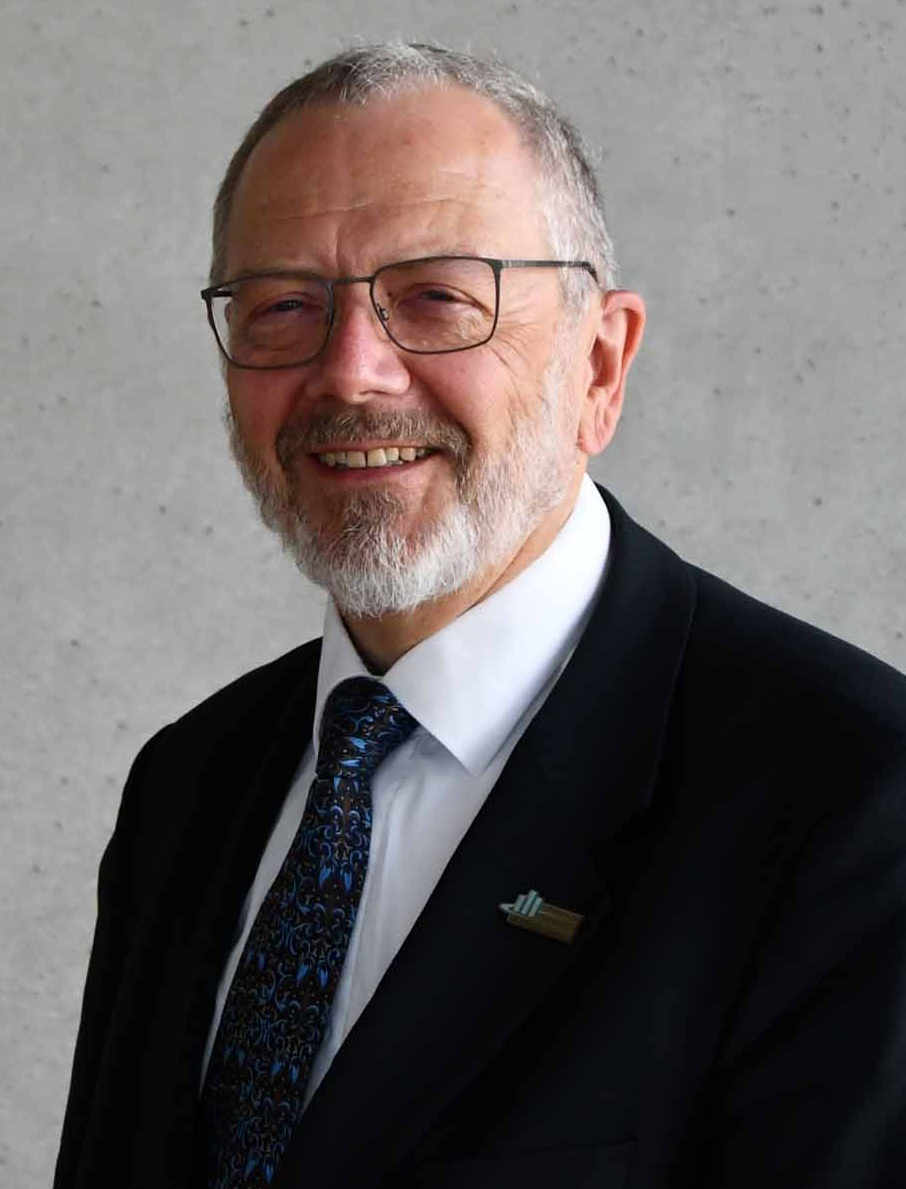
\includegraphics[width=1in,height=1.25in,clip,keepaspectratio]{Images/Wagner_Portrait.jpg}}]
{MATTHIAS WAGNER} received a Diploma and a Dr. rer.nat. in Physics from the Johannes Gutenberg - Universität Mainz (Germany). He was head of Measuring Technology Software Development at Hottinger Baldwin Messtechnik (HBM) in Darmstadt (Germany) from 1990 until 2002. In 2002, he was appointed as Professor of Computer Science at the Frankfurt University of Applied Sciences in Frankfurt am Main (Germany). Since 2005, he has been the Program Director of the international M.Sc. program “High Integrity Systems”. From 2017 to March 2020, he served as Vice-Dean for Research and International Relations of the FB2, Department of Computer Science and Engineering. Since 2010, he has been head of the Research Group Wireless Sensor Networks and Internet of Things (WSN \& IoT). His research interests cover safety critical computer systems, smart sensors and actuator networks, Software and Systems Engineering and Computational Science are supported by research stays at the UCASE Software Engineering Research Group of the Universidad de Cádiz (Spain) and the Dipartimento di Fisica e Astronomia of the Università degli Studi di Firenze (Italy). 
\end{IEEEbiography}

\begin{IEEEbiography}[{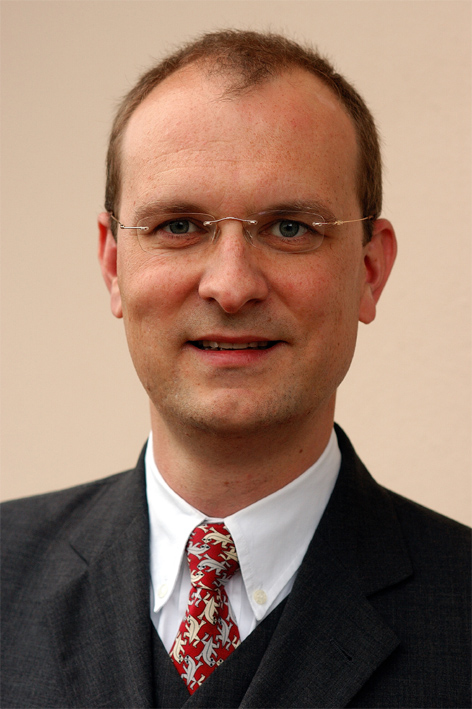
\includegraphics[width=1in,height=1.25in,clip,keepaspectratio]{Images/DSC_2004-09-26T14-30-01_mod4.jpg}}]{Jörg Schäfer} (M’12-22) is a professor of Computer Science at Frankfurt University of Applied Sciences. He received his PhD degree from Bochum University (Germany) in Mathematical Physics in 1992. After spending more than 10 years working as a principal architect in IT consulting for large international companies he was  appointed as full professor of Computer Science at Frankfurt University of Applied Sciences in 2009. Since 2012 he served as the chairman of the computer science B.Sc.\ program. 
His  main research interest is in theoretical understanding of deep learning architectures and applying machine learning and probabilistic models in ubiquitous computing applications. He runs a research group on human activity recognition (HAR) and channel state information (CSI) and jointly with Matthias Wagner and Dirk Stegelmeyer the research group industrial data science (INDAS). He is collaborating with UCASE Software Engineering Research Group of the Universidad de Cádiz (Spain). 
\end{IEEEbiography}

\begin{IEEEbiography}[{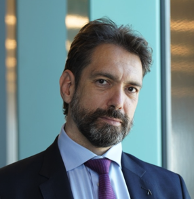
\includegraphics[width=1in,height=1.25in,clip,keepaspectratio]{Images/david.png}}]{David G\'omez-Ullate} received his PhD in Physics from Universidad Complutense de Madrid in 2001. He is a Distinguished Researcher at University of Cádiz, where he founded and serves as Director of \href{http://datalab.uca.es/}{UCA Datalab}. He is Professor of Applied Mathematics on leave from Complutense University of Madrid, Adjunct Professor at IE Business School and Visiting Professor of Mathematics and Data Science at the University of Loughborough (United Kingdom). 
His research interests span a wide range of topics, ranging from mathematical physics and approximation theory to applied machine learning and data science. His major contribution is the theory of exceptional orthogonal polynomials, which has earned him international recognition expressed as plenary talks in the main conferences of the field, and invited seminars at Cambridge, Harvard, Edinburgh, Stockholm, Copenhagen and Rome, among others. For the past 10 years he has specialized in knowledge transfer of mathematics to industry. He is currently President of the Knowledge Transfer Commission of the Royal Spanish Mathematical Society, and a member of its Governing Board. In 2016 he received a Leonardo Scholarship from the BBVA Foundation for a project on credit card fraud detection.  He has coordinated 8 knowledge transfer contracts with industry in the financial, fisheries, biomedical, legaltech and aeronautical sectors. He is co-founder and scientific advisor of the technological startup \href{https://komorebi.ai/}{Komorebi AI}.
\end{IEEEbiography}
\EOD

\end{document}
